%%% File encoding: UTF-8
%%% äöüÄÖÜß  <-- no German umlauts here? Use an UTF-8 compatible editor!

%%% Magic comments for setting the correct parameters in compatible IDEs
% !TeX encoding = utf8
% !TeX program = pdflatex 
% !TeX spellcheck = en_US
% !BIB program = biber

\RequirePackage[utf8]{inputenc} % Remove when using lualatex or xelatex!
\RequirePackage{hgbpdfa}        % Creates a PDF/A-2b compliant document

\documentclass[type=master,language=english,smartquotes]{hgbthesis}
% Supported options in [..]: 
%		Type of thesis: type = 'master' (default), 'bachelor', 'diploma', 'phd', 'internship', 'custom'
%		Theme (layout of title pages): theme=default
%		Thesis proposal: 'proposal' or 'proposal=true' 
%		Main text language: language = 'german' (default), 'english'
%		Title page language: titlelanguage = 'german', 'english' (default is main language)
%		Use automatic quotation marks: 'smartquotes'
%		Use APA citation style: 'apa'
%%%-----------------------------------------------------------------------------

\graphicspath{{images/}}  % Verzeichnis mit Bildern und Grafiken
\bibliography{references} % BibLaTeX-Literaturdatei (references.bib)

%%%-----------------------------------------------------------------------------
\begin{document}
%%%-----------------------------------------------------------------------------

%%%-----------------------------------------------------------------------------
% Title page entries
%%%-----------------------------------------------------------------------------

\title{Partial Solutions to Universal Problems}
\author{Alex A.\ Wiseguy}
\programname{Universal Computing}

%\programtype{Fachhochschul-Bachelorstudiengang} % select/edit
\programtype{Fachhochschul-Masterstudiengang}
\institution{Fachhochschule Oberösterreich}

\placeofstudy{Hagenberg}
\dateofsubmission{2024}{06}{25} % {YYYY}{MM}{DD}

\advisor{Roger K.~Putnik, M.Sc.} % optional

\license{cclicense} 			% publish under Creative Commons License (recommended)
%\license{strictlicense}	% restrictive clause - "all rights reserved"

%%%-----------------------------------------------------------------------------
\frontmatter                                   % Front part (roman page numbers)
%%%-----------------------------------------------------------------------------

\maketitle
\tableofcontents

\chapter{Preface}






 % A preface is optional
\chapter{Abstract}

\begin{english}
Large Public Display Games place a number of very specific design requirements. Such games need to work equally well for just a few or several simultaneous users. Also, the processes of entering, leaving or joining a game in progress should be easily performed without interrupting the flow of the game. This bachelor thesis focuses on the development of a framework of game mechanics that support the principle of smooth transition gameplay. This framework will then be evaluated utilizing a prototype implemented as a project in the fifth semester.
\end{english}

\chapter{Kurzfassung}

An dieser Stelle steht eine Zusammenfassung der Arbeit, Umfang
max.\ 1 Seite. Im Unterschied zu anderen Kapiteln ist die
Kurzfassung (und das Abstract) üblicherweise nicht in Abschnitte
und Unterabschnitte gegliedert. 
Auch Fußnoten sind hier falsch am Platz.

Kurzfassungen werden übrigens häufig -- zusammen mit Autor*in und Titel
der Arbeit -- %
in Literaturdatenbanken aufgenommen. Es ist daher darauf zu
achten, dass die Information in der Kurzfassung für sich 
\emph{allein} (\dah ohne weitere Teile der Arbeit) zusammenhängend und
abgeschlossen ist. Insbesondere werden an dieser Stelle (wie \ua
auch im \emph{Titel} der Arbeit und im \emph{Abstract})
normalerweise \emph{keine Literaturverweise} verwendet! Falls
unbedingt solche benötigt werden -- etwa weil die Arbeit eine
Weiterentwicklung einer bestimmten, früheren Arbeit darstellt --,
dann sind \emph{vollständige} Quellenangaben in der Kurzfassung
selbst notwendig, \zB %
[\textsc{Zobel} J.: \textit{Writing for Computer Science -- The Art of
Effective Commu\-nica\-tion}. Springer-Verlag, Singa\-pur, 1997].

Auch sollte daran gedacht werden, dass bei der Aufnahme in Datenbanken
Sonderzeichen oder etwa Aufzählungen mit "Knödellisten" in der
Regel verloren gehen. Dasselbe gilt natürlich auch für das 
\emph{Abstract}.


Inhaltlich sollte die Kurzfassung \emph{keine} Auflistung der
einzelnen Kapitel sein (dafür ist das Einleitungskapitel
vorgesehen), sondern dem*der Leser*in einen kompakten, inhaltlichen
Überblick über die gesamte Arbeit verschaffen. Der hier verwendete
Aufbau ist daher zwangsläufig anders als der in der Einleitung.


%%%-----------------------------------------------------------------------------
\mainmatter                                    % Main part (arabic page numbers)
%%%-----------------------------------------------------------------------------

\chapter{Introduction}
\label{cha:Introduction}



\chapter{Writing a Thesis}
\label{cha:TheThesis}

Every thesis%
\footnote{Most of the following remarks apply equally to bachelor's, master's,
and diploma theses.}
is different, yet good theses are usually very similar in structure, especially
in technical and natural science topics.

\section{Elements of a Thesis}

The following basic structure has proven itself as a starting point, which can,
of course, be varied and refined as desired:
%
\begin{enumerate}
	\item \textbf{Introduction and motivation}: What is the problem statement or
	task at hand, and why should someone be interested in it?
	\item \textbf{Speficiation of the topic in greater detail}: Here, the
	current state of the art of the technology or science is described, and
	existing deficits or open questions are pointed out. The direction of one's
	work is developed from this.
	\item \textbf{Own approach}: This is, of course, the core of the thesis.
	Here it is shown how the previously described task is solved and
	implemented, often in the form of a prototype. Illustrative examples
	supplement this part.
	\item \textbf{Summary}: What has been achieved, and what goals remain open?
	Which parts of the thesis are possible origins for further work?
\end{enumerate}
%
A particular dramaturgical structure of the work is also essential. Remember
that the reader usually has little time and---unlike in a novel---their
patience should not be tried. Explain already in the introduction (not in the
last chapter) how you approached the problem, your proposed solutions, and if
you successfully applied them.

Errors and dead ends may (and should) be described as well; their knowledge
often helps to avoid duplicate experiments and other errors and is thus
certainly more helpful than any whitewashing. Furthermore, it is definitely
not forbidden to express one's opinion.


\section{Language and Writing Style}

Theses are scientific works and should therefore be formulated concisely and
matter-of-factly. The author's person takes a back seat to the subject of the
work; avoid the first person or wordings such as "the author". Passive voice can
be a remedy, although it is vital to ensure that this does not result in an
overly complicated sentence structure. Also, remember that the active voice
makes writing sound stronger and more direct and helps to deliver essential
aspects more precisely.

Expressions such as colloquialisms, polemical formulations, or even irony and
cynicism are out of place, as is the excessive use of overly specific technical
terms.

Die Sprache in Abschlussarbeiten soll darüber hinaus geschlechtergerecht und
diskriminierungsfrei sein und dabei alle Menschen in ihrer Vielfalt gleichwertig
in Wort und Bild sichtbar machen. Um dies zu erreichen, bedient sich diese
Vorlage der Verwendung des Gendersterns (*). Dieser macht im Deutschen bei
Personenbezeichnungen zugleich Männer, Frauen und alle weiteren
Geschlechteridentitäten sichtbar und leistet somit auch dem gesetzlich
festgelegten Geschlechtseintrag \emph{divers} sprachlich Folge.

Furthermore, the language used in theses should be gender-inclusive and
non-discri\-minatory, making all people equally visible in their diversity,
both in words and images. In English, this includes using nouns that are not
gender-specific to refer to roles or professions, formation of phrases in a
coequal manner, and avoiding the blanket use of male or female terms.

Avoid gender-specific job titles such as "fireman" or "stewardess" and replace
them with the more neutral terms "firefighter" or "flight attendant". When
using pronouns, refrain from using "he" or "she". Replace these with the more
inclusive "they" to include people who identify as non-binary.

Also, check the writing for terms that might be considered racially
inappropriate. Expressions such as "master" and "slave" or "whitelist" and
"blacklist" might be considered offensive by certain groups of people. Keep this
in mind when naming things in the project or prototype. Especially in a
scientific thesis, the potential of language should be used to counter
stereotypical ideas about social roles.


\section{Writing a Thesis in English at a German-speaking University}
\label{sec:german}

While this template and the contained introduction should make it easy to write
a thesis entirely in English, there are still some things that have to remain in
German, should the University demand it.

The title page must usually be German and stays the same when the document is
set to English. Also, a German Kurzfassung is required together with the English
Abstract. Using a translator is a valid option for everyone who is not fluent
in German. Having the translation checked by a native German speaker is
recommended, however.

The German term "Fachhochschule" (as in Fachhochschule Oberösterreich) is
translated with "University of Applied Sciences". A master's thesis is called
"Masterarbeit," and a bachelor's thesis is called "Bachelorarbeit".

If one's native language is German, it should be considered that writing a
thesis in English (unless the program requires it) does not make writing any
easier, even if it might feel that way at first. Particularly in computer
science, the dominance of English technical terms makes writing in German seem
tedious, and switching to English might appear particularly attractive. However,
this is deceptive since one's skill in a foreign language is often overestimated
(despite the usually long years of English education). Conciseness and clarity
are easily lost, and sometimes the result is an embarrassing drivel without
context and solid content. Unless one's English skills are excellent, writing at
least the most essential parts of the thesis in German first and only
translating them afterward is advisable. Special care should be taken when
translating seemingly familiar technical terms. In addition, it is always
advisable to have the finished work checked by a native speaker.

Parallel to this document, there is also a German version, which is largely
identical in content. It contains helpful hints for writing a thesis in German
and should be used if German is the language of choice. Technically, except for
the language setting and the different quotation marks (see
Section~\ref{sec:quotation-marks}), there is nothing more to consider to use
this template in German.

\chapter{Working with \latex}
\label{cha:WorkingWithLatex}


\section{Getting Started}
\label{sec:LatexGettingStarted}

\latex is a widespread and classic document preparation system for creating
large and complicated documents with professional requirements. Working with
\latex appears---at least for inexperienced users---at first, more complex
than with conventional tools for word processing.

First, unlike most common word processors, \latex is not \textsc{WYSIWYG}.%
\footnote{"What You See Is What You Get." There were some \textsc{WYSIWYG}
editors for \latex, but they all have disappeared in the last years.}
However, it is a \emph{markup} language (like HTML) that can be somewhat
complicated for beginners together with a set of associated tools. The
supposedly strong restrictions of \latex, especially concerning the choice of
fonts and layout, certainly also seem unfamiliar. While at first, the impression
arises that this rigidity limits one's creativity, it is noticeable after a
while that it is precisely through this that one concentrates more on the
content of the work than on its outer form. The fact that the form is still
correct in the end, however, is only guaranteed if one imposes extreme
restraint on oneself when it comes to modifying the formats and parameters;
unless, of course, one has already become a \latex \emph{expert} in the
meantime.

In the end, the effort is worth it, especially since the thesis is a substantial
effort (with or without \latex). However, with the help of \latex, a
professional-looking result should be easier to achieve, and it should also save
some trouble with errors and limitations of standard software. In addition, one's
(semi-){\obnh}professional eye for the subtleties of book typesetting might
further develop along the way.%
\footnote{By the way, this final text element was set like this to enable a line
break after the parenthesis: \texttt{\ldots (semi-)\{{\bs}obnh\}professional\ldots}
The command \texttt{{\bs}obnh} ("optional break with no hyphen") is defined in
\texttt{hgbabbrev.sty}.}

\subsection{Software}
\label{sec:Software}

To work with \latex, one needs---besides a computer---the necessary software. In
the past, the individual components of \latex often had to be painstakingly
gathered and configured for one's environment. Nowadays, ready-made
distributions are available for the most important platforms (Windows, macOS,
Linux) that contain everything needed. The current version of \latex\ is
\LaTeXe\ (pronounced "LaTeX two e"). Working locally with \latex requires two
things:
%
\begin{itemize}
    \item A \latex installation (distribution).
    \item A text editor or authoring environment (front end).
\end{itemize}
%
All components are free of charge and available for all common platforms.

Alternatively, an online editor can be used, which allows working in the browser
and does not require any installation on one's computer. In addition, the work
can easily be shared with other people, such as the supervisor. Details about
recommended setups and possible alternatives can be found in
Appendix~\ref{app:TechnicalDetails}.

\subsection{Literature}
\label{sec:literature}

It is tedious to start with \latex without relevant literature; even advanced
users will often require help. Fortunately, many helpful resources are available
online. Good starting points are \eg
%
\begin{itemize}
    \item \citetitle{Oetiker2021} by \textcite{Oetiker2021} or
	\item \citetitle{Daniel2018} by \textcite{Daniel2018} (only available in German).

\end{itemize}
%
\noindent
As well-known and often referenced manual to \latex 
%
\begin{itemize}
    \item \citetitle{Kopka2003} by \textcite{Kopka2003}
\end{itemize}
%
can be recommended. Numerous other documents on \latex and related topics can be
found online at the \emph{Comprehensive TeX Archive Network} (CTAN) at
%
\begin{quote}
    \url{https://ctan.org/}
\end{quote}
%
Particularly useful are \citetitle{Pakin2021} \cite{Pakin2021} and the
descriptions of important \latex packages, such as
%
\begin{itemize}
    \item[] \texttt{babel} \cite{Bezos2023},
    \item[] \texttt{graphics}, \texttt{graphicx} \cite{Carlisle2021},
    \item[] \texttt{fancyhdr} \cite{Oostrum2022},
    \item[] \texttt{caption} \cite{Sommerfeldt2022}.
\end{itemize}


\section{Typesetting}

When working with a \latex document, one of the first things is to specify the
font used. Text passages can then be accentuated by changing the font style
using different kinds of markup.

\subsection{Fonts}

\latex normally uses the fonts of the \emph{Computer Modern} (CM) series, which,
like the \emph{TeX} software itself, were developed by Donald Knuth.%
\footnote{\url{https://www-cs-faculty.stanford.edu/~knuth/}}
The three basic CM series fonts in \latex are
%
\begin{quote}
    \begin{tabular}{lcl}
        \textrm{Roman}      & & \verb!\textrm{Roman}!,      \\
        \textsf{Sans Serif} & & \verb!\textsf{Sans Serif}!, \\
        \texttt{Typewriter} & & \verb!\texttt{Typewriter}!.
    \end{tabular}
\end{quote}
%
In the eyes of many users, the quality and timelessness of these fonts alone is
a reason to use \latex for professional purposes. Another advantage of
\emph{TeX} fonts is that the different font families and weights are very
well-matched in size.

In addition, any \emph{PostScript} font (Type 1) can be used in \latex, but this
requires some finetuning in practice. Frequently used are, \eg, \emph{Times}
and \emph{Palatino}, but there is a trend back to using the classic CM fonts.

\subsection{Text Effects}

Text can be formatted in different ways.
%
\begin{itemize}
    \item \textit{Italicization} (\verb!\textit{..}!) is especially suitable for
    emphasizing and quotations, but also for product names, foreign words, and
    mathematical variables in the text, \eg
    \begin{quote}
        \verb!\textit{Variable}! $\rightarrow$ \textit{Variable}
    \end{quote}
%
    \item \textsl{Slanted} (\verb!\textsl{..}!) denotes a slanted typeface and
    thus differs significantly from \textit{italic}; for comparison:
    \begin{quote}
        \verb!\textrm{Daimler-Chrysler}! $\rightarrow$
        \textrm{Daimler-Chrysler} \newline%
        \verb!\textsl{Daimler-Chrysler}! $\rightarrow$
        \textsl{Daimler-Chrysler} \newline%
        \verb!\textit{Daimler-Chrysler}! $\rightarrow$ \textit{Daimler-Chrysler}
    \end{quote}
%
    \item \textbf{Boldface} (\verb!\textbf{..}!) is used for \textbf{headings},
    labels of \textbf{figures} and \textbf{tables}, but only in rare cases in
    continuous text:
    \begin{quote}
        \verb!\textbf{Headings}! $\rightarrow$ \textbf{Headings}
    \end{quote}
%
    \item \emph{Emphasize} (\verb!\emph{..}!) is usually equivalent to
    \verb!\textit!, but \verb!\emph! also does the "right thing" for nested
    emphases and in combination with other font styles:
    \begin{quote}
        \setlength{\tabcolsep}{0pt}%
        \begin{tabular}{lcl}
            \verb!\textrm{You're \emph{also} here?}! & $\;\rightarrow\;$ &
            \textrm{You're \emph{also} here?} \\
            \verb!\textit{You're \emph{also} here?}! & $\;\rightarrow\;$ &
            \textit{You're \emph{also} here?} \\
            \verb!\textsl{You're \emph{also} here?}! & $\;\rightarrow\;$ &
            \textsl{You're \emph{also} here?} \\
            \verb!\textbf{You're \emph{also} here?}! & $\;\rightarrow\;$ &
            \textbf{You're \emph{also} here?} \\
            \verb!\texttt{You're \emph{also} here?}! & $\;\rightarrow\;$ &
            \texttt{You're \emph{also} here?}
        \end{tabular}
    \end{quote}
%
    \item \underline{Underlining} is a relic of the typewriter era and is
    \underline{superfluous} in modern typesetting. It should therefore be used
    only in exceptional cases, \eg
    \begin{quote}
        \verb!\underline{superfluous}!%
        \footnote{Furthermore, underlined texts are not automatically
        hyphenated.}
    \end{quote}
%
\end{itemize}


\section{Text Structure}

\latex provides several commands for structuring one's text.

\subsection{Paragraph Breaks}

Paragraphs are separated in {\latex} source text exclusively by inserting one or
more \textbf{blank lines} from each other, so \emph{no other commands} are
necessary!
%
\begin{center}
	\setlength{\fboxrule}{0.2mm}
	\setlength{\fboxsep}{2mm}
	\fbox{%
		\begin{minipage}{0.9\textwidth}
			Especially the use of \texttt{\textbackslash\textbackslash} and
			\texttt{\textbackslash{newline}} commands for line breaks is a
			common \textbf{error}. Also, the statement
			\texttt{\textbackslash{paragraph}\{\}} must \emph{not} be used
			in this context; it represents---unlike in HTML---a command for
			headings with titles in \latex\ (see below).
	\end{minipage}}
\end{center}

Usually, \latex inserts \emph{no} additional vertical spacing between
consecutive paragraphs.%
\footnote{This is the default setting in \latex. It depends on parameters
such as the document class and style used.}
However, the \emph{first} line of each paragraph (except
the first paragraph of a section) is indented to define the paragraph
boundaries. This scheme has proven successful in traditional book typesetting%
\footnote{Those who do not believe it should search their bookshelf (or their
parents' bookshelf if necessary) for counterexamples.}
and should be retained unless there are very good reasons against it. Headings
(see below) are provided for all other outlines in the vertical text flow.

\subsection{Headings}
\label{sec:headings}

\latex provides---depending on the document class used---a set of predefined
heading formats in the following order:
%
\begin{quote}
    \verb!\part{!\texttt{\em Title}\verb!}!%
    \footnote{\texttt{part} is intended for splitting a more extensive document
    into several parts and is usually not used in a thesis (and not in this
    document).}
    \newline%
    \verb!\chapter{!\texttt{\em Title}\verb!}! \newline%
    \verb!\section{!\texttt{\em Title}\verb!}! \newline%
    \verb!\subsection{!\texttt{\em Title}\verb!}! \newline%
    \verb!\subsubsection{!\texttt{\em Title}\verb!}! \newline%
    \verb!\paragraph{!\texttt{\em Title}\verb!}! \newline%
    \verb!\subparagraph{!\texttt{\em Title}\verb!}!
\end{quote}
%
\paragraph{Frequent error:} When using \verb!\paragraph{}! and
\verb!\subparagraph{}!---as seen in this paragraph---the text following the
title continues on the same line without a line break; care should be taken to
use appropriate punctuation in the title (here, \eg, \underline{\texttt{:}}).
The horizontal spacing after the title alone would not make it recognizable as a
heading.

\subsubsection{Title Capitalization}

While the English language usually only uses capital letters at the beginning of
a sentence and for proper nouns, these rules are different for titles and
headings. Varying requirements apply depending on the style guide (\eg, APA,
MLA, or The Chicago Manual of Style). While one is most welcome to delve into
these style guides, this might be too much detail when writing a thesis.
Therefore, choose one of the styles mentioned above and use a
title capitalization tool%
\footnote{\url{https://capitalizemytitle.com/} formats titles according to
several style guides, and it is easy to use.}
to get the correct output. This template uses the APA style for headings and
titles, by the way.

\subsection{Lists}

Lists are a popular means of structuring text. In \latex---similar to HTML---
three types of formatted lists are available: unordered lists ("bullet lists"),
ordered lists (enumerations), and description lists:
%
\begin{verbatim}
    \begin{itemize}     ... \end{itemize}
    \begin{enumerate}   ... \end{enumerate}
    \begin{description} ... \end{description}
\end{verbatim}
%
List entries are marked using \verb!\item!, for \texttt{description} lists with
\verb!\item[!\texttt{\em title}\verb!]!. Lists can be nested; for
\texttt{itemize} and \texttt{enumerate} lists, the bullets change with nesting
depth (see the \latex documentation for details).

\subsection{Paragraph Formatting and Line Spacing}

Theses---like books---are usually formatted in one column and justified, which
makes sense for the continuous text due to the considerable line length.
However, there are often problems with hyphenation and justification within
tables because of the small column width. Using ragged-right aligment (e.g., in
Table~\ref{tab:synthesis-techniques} on page \pageref{tab:synthesis-techniques})
is advisable in this case.

\subsection{Footnotes}

Footnotes can be placed in \latex at almost any position, but definitely in
normal paragraphs, using the command
%
\begin{quote}
    \verb!\footnote{!\texttt{\em Footnote text}\verb!}!.
\end{quote}
%
There should \emph{never be a space} between the \verb!\footnote! command and
the preceding text (comment out any line breaks with \verb!%!). The numbering
and placement of footnotes are done automatically; extensive footnotes are
wrapped on two consecutive pages if necessary.

\subsubsection{Footnotes in Headings}

This is also necessary from time to time, but is no simple case because the
footnote in a heading must only appear on the spot and not in the \emph{table
of contents}! A concrete example is the heading for Chapter~\ref{cha:Closing},
which is defined as follows:
%
\begin{quote}
    \begin{verbatim}
\chapter[Closing Remarks]%
        {Closing Remarks%
        \protect\footnote{This note ....}}%
    \end{verbatim}
\end{quote}
%
The first (optional) title \verb![Closing Remarks]! is the entry in the table of
contents and the page header. The second (identical) title \texttt{\{Closing
Remarks\}} appears on the current page and also contains the \verb!\footnote{}!
entry, which, at this point, must be "protected" by the \verb!\protect!
directive. The \verb!%! characters are necessary here to eliminate possible
spaces caused by line breaks in the source text (this trick is often needed in
\latex, see Section~\ref{sec:comments}). All in all, this is quite complicated,
and thus another reason to avoid footnotes altogether in such places.

In general, footnotes should be used sparingly, as they interrupt the flow of
the text and distract the reader. In particular, footnotes should not take up a
large part of the page and thus form a second document (as seen in some social
science publications).%
\footnote{In documents with many footnotes, this allegedly leads some readers to
the point where they regularly start reading the footnotes out of curiosity (or
by mistake) and then laboriously search for the associated small-print
references in the main text.}

\subsection{Cross-References}
\label{sec:cross-references}

To manage cross-references within a document, \latex\ provides a straightforward
mechanism. First, each location (chapter, section, figure, table, \etc) must be
marked by
%
\begin{quote}
    \verb!\label{!\texttt{\em key}\verb!}!
\end{quote}
%
where \texttt{\em key} must be a valid \latex symbol.
To prevent confusion about labels (which are just numbers), it is common to give
them a different prefix depending on their meaning, \eg
%
\begin{quote}
    \tabcolsep0pt
    \begin{tabular}{ll}
        \verb!cha:!\texttt{\em chapter} & \ \ldots\ for chapters, \\
        \verb!sec:!\texttt{\em section} & \ \ldots\ for sections and
        subsections, \\
        \verb!fig:!\texttt{\em figure} & \ \ldots\ for figures, \\
        \verb!tab:!\texttt{\em table} & \ \ldots\ for tables, \\
        \verb!equ:!\texttt{\em equation} & \ \ldots\ for formulae and equations.
    \end{tabular}
\end{quote}
%
\noindent
Examples:\ \verb!\label{cha:Introduction}! or \verb!\label{fig:Screen-1}!.
Using the commands
%
\begin{quote}
    \verb!\ref{!\texttt{\emph{key}}\verb!}!
    \hspace{1em} or \hspace{1em}
    \verb!\pageref{!\texttt{\emph{key}}\verb!}!
\end{quote}
%
allows the number or page number associated with \texttt{\emph{key}} to be
inserted anywhere in the document, \eg
%
\begin{quote}
    \verb!.. as mentioned in Chapter~\ref{cha:Introduction} ..!\\
    \verb!.. the screenshot on page \pageref{fig:Screen-1} ..!
\end{quote}
%
By the way, the terms \emph{chapter} and \emph{section} are frequently misused.
Chapters always have whole numbers:
%
\begin{quote}
    \begin{tabular}{ll}
        \textrm{Correct:\ } & Chapter 7 or Section 2.3.4 \\
        \textbf{Incorrect:\ }  & Chapter 7.2 or Section 5
    \end{tabular}
\end{quote}

\emph{Chapter} and \emph{Section}, as well as \emph{Figure}, \emph{Table},
\emph{Listing}, or \emph{Equation}, should always be capitalized when used in
connection with a cross-reference.
%
\begin{quote}
	\begin{tabular}{ll}
		\textrm{Correct:\ } & \ldots\ see Figure 4.1 \ldots\ as stated in
		Chapter 4 \ldots \\
		\textbf{Incorrect:\ }  & \ldots\ see figure 4.1 \ldots\ as stated in
		chapter 4 \ldots
	\end{tabular}
\end{quote}

\subsection{Hyperlinks and E-mail Addresses}

Hyperlinks (URLs) present a particular challenge for typesetting, especially
when a line break occurs. The command
%
\begin{quote}
    \verb!\url{!\texttt{\em address}\verb!}!
\end{quote}
%
allows wrapping at certain address characters and should always be used when a
hyperlink is specified in the body text or within a footnote.

For e-mail addresses the macro
%
\begin{quote}
    \verb!\email{!\texttt{\em e-mail address}\verb!}!
\end{quote}
%
was defined in \texttt{hgb.sty}. It creates a correct link in the document with
a \texttt{mailto:} prefix using \verb|\url{}|. The statement can also be used
within the \verb|\author{}| command in the preamble of a document to
additionally specify an e-mail address on the title page:
%
\begin{quote}
    \begin{verbatim}
\author{%
    Alex A. Wiseguy \\%
    \email{alex@wiseguy.org}%
}
    \end{verbatim}
\end{quote}
%


\section{Word Spacing and Punctuation}

While \latex automatically tries to achieve the best possible result in many
typesetting areas, punctuation requires the author's care.

\subsection{\emph{French Spacing}}

In English-language typesetting, it is customary to insert an increased space
(compared to the usual space between words) after the end each sentence.
Although this is not enabled by default for this document (it is also not
traditionally done in German and French), it is sometimes preferred because of
improved readability. If the English ("non-French") sentence separation with
additional spacing is desired, only the line
%
\begin{quote}
    \verb!\nonfrenchspacing!
\end{quote}
%
needs to be added at the beginning of the document. In this case, however, the
punctuation within sentences (after .\ and :) should be carefully observed. For
example, "Dr.\ Mabuse" is written in the form
%
\begin{quote}
    \verb!Dr.\ Mabuse! or \verb!Dr.~Mabuse!
\end{quote}
%
In the second example, the \verb!~! character also prevents a line break at the
space character.

\subsection{Dashes and Hyphens}
\label{sec:dash}

Confusing dashes with hyphens or similar punctuation marks (with and without
spaces) are common errors. The following different types need to be
distinguished:
%
\begin{itemize}
    \item Hyphens (as in "tech-savvy").
    \item Minus signs, \eg $-7$ (created with \verb!$-7$!).
    \item Dashes---such as the em dash here (generated with \verb!---!).
\end{itemize}
%
\noindent
Dashes are used for pauses or indicating ranges. There are clear conventions
for using them:%
\footnote{Both versions also have corresponding special characters in
\emph{Word}.}
%
\begin{enumerate}
	\item In \emph{English} texts, the \emph{em dash} is used \emph{without}
	extra spaces---\emph{as we should know by now} (in \latex by typing
	{\verb*!---!}).
	\item In \emph{German}, the slightly shorter \emph{en dash} surrounded by
	two spaces is usually used -- wie hier zu sehen (in \latex by typing
	{\verb*! -- !})). This dash is also used in both languages to indicate
	intervals of numbers (pages 12--19), but in this case without spaces.
\end{enumerate}

\subsection{Comments}
\label{sec:comments}

Text parts can be commented out line by line in \latex\ with \verb!%!. The text
after a \verb!%! character is ignored until the subsequent end-of-line:
%
\begin{quote}
    \verb!This will be printed. %This text will be ignored.!
\end{quote}
%
Comment characters are frequently used to hide \emph{white space}, \ie, spaces
and line breaks. The following example shows how \verb!%! at the end of a line
can be used to avoid the occurrence of a space before a subsequent footnote
marker:
%
\begin{quote}
\begin{verbatim}
In Austria, people eat schnitzel on Sundays.%
\footnote{Which explains the generally good condition.}
\end{verbatim}
\end{quote}
%
Similarly, the occurrence of unwanted paragraph space can be avoided by the
selective use of comment lines,\eg, before and after a centered text section:
%
\begin{quote}
\begin{verbatim}
... normal text.
%
\begin{center}
   This test is centered.
\end{center}
%
And now it continues normally ...
\end{verbatim}
\end{quote}
%
In addition, the \verb!comment! environment offers the possibility to hide
larger text blocks in one piece:
%
\begin{quote}
\begin{verbatim}
\begin{comment}
This text ...
   ... is ignored.
\end{comment}
\end{verbatim}
\end{quote}

\subsection{Quotation Marks}
\label{sec:quotation-marks}

Quotation marks are a common (and often unnoticed) source of error; again, the
differences between English and German (among other languages) should be noted.

\subsubsection{Variant 1: Quotation Marks Using \latex's Default Setting}

With \latex's default setting (\ie, \emph{without} using the document option
\texttt{smartquotes} set here, see below), typing the leading and trailing
quotation marks must strictly follow the appropriate conventions. Here is the
correct \latex notation for English and German texts:
%
\begin{quote}
    \verb!``English''! $\rightarrow$ ``English'',\\
    \verb!"`Deutsch"'! $\rightarrow$ {\glqq}Deutsch{\grqq}.
\end{quote}
%
Note the subtle typographical differences between the two languages.%
\footnote{Some editors (\eg, \textsf{TeXstudio}) can be configured to use the
corresponding quotation marks \emph{automatically} (context- and
language-dependent) when typing a double quote character
(\texttt{\textquotedbl}). However, this is currently not possible in
\textsf{Overleaf}.}

\emph{Single} quotation marks are generated analogously in English. In German,
however, the macros \verb!\glq! and \verb!\grq! (German left/right quote) are
required:
%
\begin{quote}
    \verb!`English'! $\rightarrow$ `English',\\
    \verb!{\glq}Deutsch{\grq}! $\rightarrow$ {\glq}Deutsch{\grq}.
\end{quote}

\subsubsection{Variant 2: Quotation Marks Using the Option \texttt{smartquotes}}

By setting the \texttt{smartquotes} document option, this template uses a
\emph{particular setup} based on the \texttt{csquotes} package.%
\footnote{\url{https://ctan.org/pkg/csquotes}}
This significantly simplifies the right use of quotation marks because the
correct character is used depending on the current language setting and the
position of the quote character. It is sufficient to use a double quote
character \texttt{\textquotedbl} to achieve this:
%
\begin{quote}
	\verb!"English"! $\rightarrow$ "English" (with language setting
	\texttt{english})\\
	\begin{german}%
		\verb!"Deutsch"! $\rightarrow$ "Deutsch"
	\end{german}
	(with language setting \texttt{german})
\end{quote}
%
It should be noted that the standard input of quotation marks (variant~1, see
above) is \emph{not} available in this case. The combined use of variant~1 and
variant~2 is thus not possible! With this setting, also all other shorthands of
the \texttt{babel} package%
\footnote{\url{https://ctan.org/pkg/babel}}
(like, e.g., \verb!"a!, \verb!"o!, \verb!"u!) are \emph{permanently disabled},
and they cannot be reactivated locally either.%
\footnote{The use of the \texttt{\textquotedbl} character as the double-sided
"outer quote" character is considered "dangerous"---especially in combination
with the German language---because the \texttt{babel} package uses the double
quote character for special \emph{shorthand} macros. We bravely accept this,
though the \texttt{babel}-shorthands are generally disabled in the current
setup to avoid trouble.}

\subsubsection{Additional Features of the \texttt{csquotes} Package}

The \texttt{csquotes} package (automatically loaded with the
\texttt{smartquotes} option) provides many more possibilities for entering
quoted text (quotations), especially the command
%
\begin{itemize}
    \item[] \verb!\enquote{text}!,
\end{itemize}
%
which uses the given \texttt{text} in the correct form (among other things
depending on the language setting and nesting depth) as a citation, \eg
%
\begin{itemize}
    \item[] \verb|\enquote{I have a dream.}|
    \item[] $\rightarrow$ \enquote{I have a dream.}
\end{itemize}
%
The advantage of this construct is especially apparent in \emph{nested}
quotations, as, for example in
%
\begin{itemize}
    \item[] \verb|\enquote{Napoleon just said \enquote{Keep going!} and left.}|
    \item[] $\rightarrow$ \enquote{Napoleon just said \enquote{Keep going!} and
    left.}
\end{itemize}
%
Another handy feature is the command \verb!\foreignquote! which makes it very
easy to insert foreign quotations in the text without explicitly changing the
language setting, \eg%
\footnote{Currently only the language settings \texttt{english} and
\texttt{german} are available.}
%
\begin{itemize}
    \item[] \verb|\foreignquote{german}{Da sprach der Herr zu Kain:|\newline
    \verb|   \enquote{Wo ist dein Bruder Abel?} Er entgegnete: \ldots}|
    \item[] $\rightarrow$ \foreignquote{german}{Da sprach der Herr zu Kain:
    \enquote{Wo ist dein Bruder Abel?}  Er entgegnete: \ldots}
\end{itemize}


\section{Hyphenation}
\label{subsec:hyphenation}

Hyphenation is essential to achieve a clean typeface, especially for long words.
It is done either \emph{automatically} or \emph{manually} by inserting optional
hyphens.

\subsection{Automatic Line Break}

In \latex, hyphenation is always performed automatically. The language is set at
the beginning of the document, and appropriate hyphenation rules are applied to
the entire text.

Especially for narrow text columns, \latex may not find a suitable place for the
line break and lets the text run beyond the right margin. This is intentional
and meant to indicate a problem that needs to be repaired through manual
intervention.

\subsection{Manual Line Break}

Generally, one should be suspicious of the automatic hyphenation and always
check the final result carefully. Especially words with umlauts or compound
words with hyphens (see below) are often split incorrectly in \latex.

\paragraph{Optional line breaks:} If required, specific allowed hyphenation
points can be defined with \verb!\-!, as for example in
%
\begin{itemize}
    \item[] \verb!in\-com\-pre\-hen\-si\-ble!.
\end{itemize}

\paragraph{Compound words:} An unpleasant peculiarity of \latex is that in
\emph{hyphenated} words, the individual parts of words are generally \emph{not
automatically} hyphenated! This is quite common, especially (but not only) in
German texts, and thus annoying; for example, \latex will not hyphenate
\emph{either} of the two parts of the word
%
\begin{itemize}
    \item[] \verb!anti-intellectualism!
\end{itemize}
%
but if necessary, let it run beyond the right margin! Manual hyphenation through
inserting \verb!\-! can once again be helpful.

\paragraph{"Sloppy" formatting:} In real problem cases---for example, text
elements that must not or cannot be wrapped---\latex\ can be told to be less
strict about formatting specific paragraphs. This is achieved as follows:
%
\begin{LaTeXCode}[numbers=none]
\begin{sloppypar}
    This paragraph is set "sloppy" ...
\end{sloppypar}
\end{LaTeXCode}
%
The last resort is to rewrite the passage in question in such a way that it
results in a decent line break---after all, it is one's own work, and no
justification is owed to anyone (apart maybe from the supervisor).%
\footnote{It is said that independent changes to the text by typesetters were
also quite common in the metal type days.}


\section{The \texttt{hagenberg-thesis} Package}

This package contains several \latex\ files that are required to create this
document:
%
\begin{itemize}
    \item \nolinkurl{hgbthesis.cls} (class file): Defines the document
    structure, layout, and the entire preamble of the document (title page,
    \etc).
    \item \nolinkurl{hgb.sty} (style file): Contains central definitions and
    settings. This file is automatically loaded by \nolinkurl{hgbthesis.cls},
    but it can also be used for other documents.
    \item Additional style files imported by \nolinkurl{hgbthesis.cls}:
    \begin{itemize}
        \item[] \nolinkurl{hgbabbrev.sty} (various abbreviations)
        \item[] \nolinkurl{hgbalgo.sty} (algorithms)
        \item[] \nolinkurl{hgbbib.sty} (reference management)
        \item[] \nolinkurl{hgbheadings.sty} (page headers)
        \item[] \nolinkurl{hgblistings.sty} (code listings)
        \item[] \nolinkurl{hgbmath.sty} (mathematical functionalities)
    \end{itemize}
\end{itemize}


\subsection{Settings}
\label{sec:hagenberg-settings}

All (\verb!.tex!) documents of this package start with the statement
%
\begin{itemize}
    \item[] \verb!\documentclass[!\texttt{\emph{type}},
    \texttt{\emph{language}}\verb!]{hgbthesis}!.
\end{itemize}
%
The \texttt{\emph{type}} option specifies the type of document:
%
\begin{itemize}
    \item[] \texttt{master} (master thesis = \emph{default})
    \item[] \texttt{diploma} (diploma thesis)
    \item[] \texttt{bachelor} (bachelor thesis)
    \item[] \texttt{internship} (internship report)
	\item[] \texttt{proposal} (exposé, in connection with \texttt{bachelor} or
	\texttt{master})
\end{itemize}
%
The \texttt{\emph{language}} option can be used to specify the primary language
of the document; possible values are:
%
\begin{itemize}
    \item[] \texttt{german} (\emph{default})
    \item[] \texttt{english}
\end{itemize}
%
Additional options:
%
\begin{itemize}
    \item[] \texttt{smartquotes} (use of regular double quotes, see
    Section~\ref{sec:quotation-marks}).
\end{itemize}
%
If \emph{no} option is specified, the default is \texttt{[master,german]}. The
full source code for a corresponding \verb!.tex! main file is listed in
Appendix~\ref{app:latex}.

\subsubsection{Details of the Thesis or Report}

The document class is intended for different types of works that differ only in
the structure of the title pages. Different elements are required for the title
pages depending on the selected document type (see
Table~\ref{tab:TitleElements}). The following information is required for
\textbf{all} document types:
%
\begin{itemize}
    \item[] %
    \verb!\title{!\texttt{\em Thesis or report title}\verb!}!, \newline%
    \verb!\author{!\texttt{\em Author}\verb!}!, \newline%
    \verb!\programtype{!\texttt{\em Type of program}\verb!}!, \newline%
    \verb!\programname{!\texttt{\em Program}\verb!}!, \newline%
    \verb!\placeofstudy{!\texttt{\em Place of study}\verb!}!, \newline%
    \verb!\dateofsubmission{!\texttt{\em yyyy}\verb!}{!\texttt{\em
    mm}\verb!}{!\texttt{\em dd}\verb!}!, \newline%
    \verb!\advisor{!\texttt{\em Supervisor name}\verb!}! --
    optional.
\end{itemize}
%
\noindent
For \textbf{internship reports}, the following elements are considered in
addition to the basic information:
%
\begin{itemize}
    \item[] %
    \verb!\companyName{!\texttt{\em Name and address of the company}\verb!}!
    \newline%
    \verb!\companyUrl{!\texttt{\em Company website}\verb!}!
\end{itemize}

\begin{table}
    \caption{Elements in title pages for different document options.}
    \label{tab:TitleElements}
    \centering\small
    \begin{tabular}{@{}lcccc@{}}
        \toprule
        \emph{Element} & \texttt{master} & \texttt{bachelor} & 
				\texttt{diploma} & \texttt{internship} \\
        \midrule
        \verb!\title!            & $+$ & $+$ & $+$ & $+$ \\
        \verb!\author!           & $+$ & $+$ & $+$ & $+$ \\
        \verb!\programtype!      & $+$ & $+$ & $+$ & $+$ \\
        \verb!\programname!      & $+$ & $+$ & $+$ & $+$ \\
        \verb!\placeofstudy!     & $+$ & $+$ & $+$ & $+$ \\
        \verb!\dateofsubmission! & $+$ & $+$ & $+$ & $+$ \\
        \verb!\advisor!          & $+$ & $+$ & $+$ & $+$ \\
        \verb!\companyName!      & $-$ & $-$ & $-$ & $+$ \\
        \verb!\companyPhone!     & $-$ & $-$ & $-$ & $+$ \\
        \bottomrule
    \end{tabular}
\end{table}

\subsubsection{Title Pages}

The first pages of the work, including the title page, are created by the
command
%
\begin{itemize}
    \item[] \verb!\maketitle!
\end{itemize}
%
depending on the above settings:
%
\begin{center}
    \begin{tabular}{@{}cl@{}}
        \toprule
        \emph{Page} & \emph{Content} \\
        \midrule
        \textrm{i}   & Title page \\
        \textrm{ii}  & Advisor page (only when \verb!\advisor! is specified) \\
        \textrm{iii} & Copyright page \\
        \textrm{iv}  & Affidavit \\
        \bottomrule
    \end{tabular}
\end{center}
%
The copyright page%
\footnote{If the \texttt{proposal} option is used, the pages for copyright and
affidavit are omitted.}
also notes the conditions for the use and distribution of the work. The
following settings can determine the associated text at the beginning of the
document.
%
\begin{description}
    \item[\normalfont\texttt{{\bs}cclicense}] ~ \newline
    Publication under a Creative Commons license%
    \footnote{\url{https://creativecommons.org/licenses/by-nc-nd/4.0/}}
    that permits free redistribution of the work with attribution to the author,
    but no commercial use or adaptation. This is the \emph{recommended} default
    setting.
    \item[\normalfont\texttt{{\bs}strictlicense}] ~ \newline
    Classic restriction of usage rights (\emph{All Rights Reserved}).
    \item[\normalfont\texttt{{\bs}license\{\emph{License text}\}}] ~ \newline
    If necessary, this can specify an alternative \text{\emph{license text}}.
    Such changes should, of course, be coordinated with the university.
\end{description}

\subsection{Defined Abbreviations}

There are also several abbreviation commands%
\footnote{Similar to the \texttt{jkthesis} style by J. Küpper
(\url{https://ctan.org/pkg/jkthesis}).}
defined in the \texttt{hagenberg-thesis} package, which simplify writing and
provide consistent spacing (Table~\ref{tab:abbreviations}). When using any
command, it should generally be noted that they sometimes "gobble" trailing
spaces so that no spacing is created before the subsequent text.%
\footnote{However, for almost all macros defined in \texttt{hgbabbrev.sty} this
is prevented by the use of \texttt{\textbackslash xspace}.}
If necessary, this can be prevented with a subsequent "\verb!\ !" or by wrapping
the expression in \verb!{}! brackets. When using commands with a trailing period
at the end of a sentence, care should also be taken to avoid \emph{double}
periods.


\begin{table}
    \caption{English and German abbreviation commands defined in
    \texttt{hgbabbrev.sty}.}
    \label{tab:abbreviations}
    \centering\small
    \begin{tabular}{@{}llp{2cm}ll@{}}
        \toprule
        \verb+\ie+   & \ie   & & \verb+\eg+  & \eg  \\
        \verb+\wrt+  & \wrt  & & \verb+\Eg+  & \Eg  \\
        \midrule
        \verb+\bzw+  & \bzw  & & \verb+\ua+  & \ua  \\
        \verb+\bzgl+ & \bzgl & & \verb+\Ua+  & \Ua  \\
        \verb+\ca+   & \ca   & & \verb+\uae+ & \uae \\
        \verb+\dah+  & \dah  & & \verb+\usw+ & \usw \\
        \verb+\Dah+  & \Dah  & & \verb+\uva+ & \uva \\
        \verb+\ds+   & \ds   & & \verb+\uvm+ & \uvm \\
        \verb+\evtl+ & \evtl & & \verb+\va+  & \va  \\
        \verb+\ia+   & \ia   & & \verb+\vgl+ & \vgl \\
        \verb+\sa+   & \sa   & & \verb+\zB+  & \zB  \\
        \verb+\so+   & \so   & & \verb+\ZB+  & \ZB  \\
        \verb+\su+   & \su   & & \verb+\etc+ & \etc \\
        \bottomrule
    \end{tabular}
\end{table}

\subsection{Language Switching}
\label{sec:language-switching}

For German-language sections (\eg, the Kurzfassung or German quotations), the
\emph{language} should be switched from English to German to get the correct
hyphenation. To avoid accidentally forgetting to reset the language, two special
\emph{environments} are provided for this purpose:
%
\begin{LaTeXCode}[numbers=none]
\begin{german}
    An dieser Stelle steht eine Zusammenfassung der Arbeit.
\end{german}
\end{LaTeXCode}
%
or respectively
%
\begin{LaTeXCode}[numbers=none]
\begin{english}
    Text in English (if the main language is set to German).
\end{english}
\end{LaTeXCode}
%
The current language setting can be displayed with the command
\verb!\languagename!. At this point, this results in
"\texttt{\languagename}".

\subsection{Additional \latex\ Packages}

Several additional \latex\ packages are required to use this document
(Table~\ref{tab:packages}). These packages are automatically loaded by the
\texttt{hagenberg-thesis} package. All packages used are part of the \latex\
standard installation, as, for example, in MikTeX, where corresponding
documentation can also be found (mainly as DVI files). The current versions of
the packages are available online on the CTAN sites given in
Section~\ref{sec:literature}.

\begin{table}
    \caption{The most important of the \latex extensions used in the
    \texttt{hagenberg-thesis} package. These are already included in typical
    \latex\ standard installations (\eg, MikTeX).}
    \label{tab:packages}
    \centering\small
    \begin{tabular}{@{}ll@{}}
        \toprule
        \emph{Package}        & \emph{Function} \\
        \midrule
        \texttt{algorithmicx} & Description of algorithms \\
        \texttt{amsfonts},
        \texttt{amsbsy}       & Mathematical symbols \\
        \texttt{amsmath}      & Mathematical typesetting \\
        \texttt{babel}        & Language switching \\
        \texttt{biblatex}     & Bibliography management \\
        \texttt{caption}      & More flexible captions \\
        \texttt{csquotes}     & Context-sensitive quotation marks \\
        \texttt{eurosym}      & {\euro} symbol (\verb!\euro!) \\
        \texttt{exscale}      & Correct font sizes in math mode \\
        \texttt{fancyhdr}     & Controlling headers and footers \\
        \texttt{float}        & Improved float handling \\
        \texttt{fontenc}      & Use of T1 (Western European) character encoding \\
        \texttt{graphicx}     & Including of graphics \\
        \texttt{hyperref}     & Handling of cross-references in the PDF doucument \\
        \texttt{ifthen},
        \texttt{xifthen}      & Conditional commands in \latex \\
        \texttt{inputenc}     & Extended input encodings \\
        \texttt{listings}     & Code listings \\
        \texttt{upquote}      & Realistic quotes in \texttt{verbatim} texts \\
        \texttt{url}          & URL handling in text \\
        \texttt{verbatim}     & Better \texttt{verbatim} environments \\
        \texttt{xcolor}       & Colored text elements and background colors \\
        \bottomrule
    \end{tabular}
\end{table}


\section{\latex\ Error Messages and Warnings}

During a run \latex\ outputs tons of messages, which should not lead to
confusion due to their abundance, e.g.:

\begin{scriptsize}
\begin{verbatim}
...
Underfull \hbox (badness 2744) in paragraph at lines 568--572
\T1/lmr/m/n/10.95 be-tween in-di-vid-ual
[]
Underfull \hbox (badness 5607) in paragraph at lines 580--581
\T1/lmr/m/n/10.95 only as a place-
[]
...
\end{verbatim}
\end{scriptsize}
%
\emph{Errors} must be corrected, but \latex\ does not make this job easy.
Sometimes (\eg, when a closing bracket \verb!}! was forgotten), the problem is
not located until much later in the text. In such cases, inspecting the
generated output document can be useful to determine at what point the results
get out of hand. In case of capital errors, the \latex processor stops
completely and does not generate any output (usually in connection with a mostly
 cryptic error message). In this case, a detailed analysis of the source code or
 the steps just performed before will usually help. A detailed error log can be
 found in the \verb!.log! file of the main document.

If no errors are shown, at least the syntactical structure of the document is
okay. However, one should take a closer look at the list of messages at the
latest when finishing the thesis. This is highly recommended to eliminate any
remaining problems, such as overlong lines of text (overfull boxes), unresolved
references, or similar issues. In any case, the result should look like this in
the end:
%
\begin{quote}
    \verb!LaTeX-Result: 0 Error(s), 0 Warning(s), ...!
\end{quote}

\chapter{Figures, Tables, Source Code}
\label{cha:Figures}

\chapter[Mathematical Formulas etc.]{Mathematical Formulas, Equations and Algorithms}
\label{cha:Mathematics}


Typesetting mathematical elements is certainly one of the strongest features of
\latex. A distinction is made between mathematical elements in continuous text
and free-standing equations, which are usually numbered consecutively.
Analogous to figures and tables, this makes it easy to cross-reference equations.
Here are only some examples and special topics, much more can be found in 
\cite[Ch.\ 7]{Kopka2003} and~\cite{Voss2014}.


\section{Mathematical Elements in Continuous Text}

Mathematical symbols, expressions, equations, etc.\ are marked in the continuous
text by pairs \verb!$! \ldots \verb!$!. Here is an example:
%
\begin{quote}
	%\item[]
	The near infinity point is at $\bar{a} = f \cdot (f / (K \cdot u_{\max}) + 1)$, 
	so with a lens set to $\infty$, everything is in focus from distance $\bar{a}$ on.
	Focusing the lens to the distance $\bar{a}$ (\ie, $a_0 = \bar{a}$), everything
	in the range $[\frac{\bar{a}}{2}, \infty]$ will be in focus.
\end{quote}
%
It is important to ensure that the height of the individual math items in the text
does not become too large.

\subsubsection{Common Mistakes}

In continuous text, simple variables are often typeset with plain text,
\ie, without using correct mathematical symbols, as in "X-axis" instead of 
"$X$-axis" (\verb!$X$-axis!).


\subsubsection{Mathematical Fonts}

\latex\ uses slightly different fonts for regular text and in math mode.
The following basic math fonts are available:
%
\begin{quote}
    \begin{tabular}{lcl}
        $\mathrm{Roman}$      & & \verb!$\mathrm{Roman}$!,      \\
				$\mathit{Italic}$     & & \verb!$\mathit{Italic}$!,      \\
				$\mathbf{Bold}$     	& & \verb!$\mathit{Bold}$!,      \\
        $\mathsf{Sans Serif}$ & & \verb!$\mathsf{Sans Serif}$!, \\
        $\mathtt{Typewriter}$ & & \verb!$\mathttt{Typewriter}$!, \\
				$\mathcal{CALLIGRAPHIC}$ & & \verb!$\mathcal{CALLIGRAPHIC}$!,\\
				$\mathbb{BLACKBOARD}$ & & \verb!$\mathbb{BLACKBOARD}$!,\\
				$\mathfrak{Fraktur}$ & & \verb!$\mathfrak{Fraktur}$!.
    \end{tabular}
\end{quote}
%
In some situations, the \verb!\boldsymbol{..}! macro may come in useful. It can 
convert any mathematical symbol into a boldface version, for example,
$\mathbf{A}$ (\verb!$\mathbf{A}$!) denotes a matrix and $\boldsymbol{x}$ 
(\verb!$\boldsymbol{x}$!) is a vector.


\subsubsection{Line Breaks}

With longer mathematical elements in the continuous text problems with line breaks 
are inevitable. Usually \latex allows line breaks only at the "=" operator, 
elsewhere one can use \verb|\allowbreak| to enable line breaks. Here is a small
example:
%
\begin{itemize}
	\item[a)] For example, (bla bla bla) a simple row vector is defined in the form
	$\boldsymbol{x} = (x_0, x_1, \ldots, x_{n-1})$.
	\item[b)] For example, (bla bla bla) a simple row vector is defined in the form
	$\boldsymbol{x} = (x_0,\allowbreak x_1,\allowbreak\ldots,\allowbreak
	x_{n-1})$.
\end{itemize}
%
The line in a) should extend beyond the page margin, but b) contains 
\verb|\allowbreak| in several places and should therefore wrap cleanly.


\section{Displayed Expressions and Equations}

Displayed mathematical expressions can be generated in \latex\ by \verb!\[! \ldots 
\verb!\]! The result will be centered, but will not be numbered.
For example, \[y_0 = 4 x^2\] is produced by \verb!\[y_0 = 4 x^2\]!
or, alternatively,
%
\begin{LaTeXCode}[numbers=none]
\begin{displaymath} y_0 = 4 x^2 \end{displaymath}
\end{LaTeXCode}



\subsection{Numbered Equations}

However, most often in such cases the \texttt{equation} environment is used
to produce numbered equations that can be referred to at any time in the text.
For example, 
%
\begin{LaTeXCode}[numbers=none]
\begin{equation}
	f(k) = \frac{1}{N} \sum_{i=0}^{k-1} i^2 .
	\label{eq:MyFirstEquation}
\end{equation}
\end{LaTeXCode}
%
creates this equation:
%
\begin{equation}
	f(k) = \frac{1}{N} \sum_{i=0}^{k-1} i^2 .
	\label{eq:MyFirstEquation}
\end{equation}
%
With \verb|\ref{eq:MyFirstEquation}| you get the number (\ref{eq:MyFirstEquation})
of this equation as usual (see also Section~\ref{sec:ReferencesToEquations}).
The same equation \emph{without} numbering can be generated with the \texttt{equation*}
environment.
%
\begin{center}
	\setlength{\fboxrule}{0.2mm}
	\setlength{\fboxsep}{2mm}
	\fbox{%
		\begin{minipage}{0.9\textwidth}
		Note that \emph{equations} are a \emph{part of the main text} in terms of content, 
		and therefore, in addition to proper linguistic \emph{transitions},
		\emph{punctuation} (as shown in Equation \ref{eq:MyFirstEquation}) must be observed.
		If you are unsure, you should look at suitable examples in a good math textbook.
		\end{minipage}}
\end{center}
%
For those interested, more on the intimate connection between mathematics and prose can
be found in \cite{Mermin1989} and \cite{Higham2020}.


\subsection{Multiline Equations}

For multiline equations \latex\ offers the \verb!eqnarray! environment which, however,
generates somewhat idiosyncratic spacing. It is recommended to use the extended
possibilities of the \texttt{amsmath} package%
\footnote{American Mathematical Society (AMS). \texttt{amsmath} is part of the 
\latex\ default installation and is automatically imported by \texttt{hgb.sty}.}
for this right away. Here is an example with two equations aligned to the $=$ sign,
%
\begin{align}
	f_1 (x,y) &= \frac{1}{1-x} + y , \label{eq:f1} \\
	f_2 (x,y) &= \frac{1}{1+y} - x , \label{eq:f2}
\end{align}
%
generated with the \texttt{align} environment from the \texttt{amsmath} package:
%
\begin{LaTeXCode}[numbers=none]
\begin{align}
  f_1 (x,y) &= \frac{1}{1-x} + y , \label{eq:f1} \\
  f_2 (x,y) &= \frac{1}{1+y} - x , \label{eq:f2}
\end{align}
\end{LaTeXCode}


\subsection{Multi-Case Constructs}

With the \texttt{cases} environment from \texttt{amsmath}, case distinctions, 
\eg, in function definitions, are very easy to accomplish.
For instance, the recursive definition
%
\begin{equation}
	f(i) =
	\begin{cases}
		0             & \text{for $i = 0$,}\\
		f(i-1) + f(i) & \text{for $i > 0$.}
	\end{cases}
\end{equation}%
%
was produced with the following commands:
%
\begin{LaTeXCode}[numbers=none]
\begin{equation}
	f(i) =
	\begin{cases}
	  0             & \text{for $i = 0$,}\\
	  f(i-1) + f(i) & \text{for $i > 0$.}
	\end{cases}
\end{equation}
\end{LaTeXCode}
%
Note the use of the very handy \verb!\text{..}! macro, which can be used
to insert ordinary text in math mode, and again the punctuation within the
equation.


\subsection{Equations With Matrices}

Again, \texttt{amsmath} offers some advantages over using the standard \latex
constructs. For this purpose, a simple example of using the \texttt{pmatrix}
environment for vectors and matrices,
%
\begin{equation}
	\begin{pmatrix}
		x' \\ y'
	\end{pmatrix}
	=
	\begin{pmatrix}
		\cos \phi & -\sin \phi           \\
		\sin \phi & \phantom{-}\cos \phi
	\end{pmatrix}
	\cdot
	\begin{pmatrix}
		x \\ y
	\end{pmatrix} ,
\end{equation}
%
generated with the following instructions:
%
\begin{LaTeXCode}
\begin{equation}
	\begin{pmatrix} 
			x' \\ 
			y' 
	\end{pmatrix}
	= 
	\begin{pmatrix}
		  \cos \phi &          -\sin \phi \\
		  \sin \phi & \phantom{-}\cos \phi /+ \label{lin:phantom} +/
	\end{pmatrix} 
	\cdot
	\begin{pmatrix} 
			x \\ 
			y 
	\end{pmatrix} ,
\end{equation}
\end{LaTeXCode}
%
A useful detail in this is the \tex macro \verb!\phantom{..}! (in line 
\ref{lin:phantom}), which inserts its argument invisibly and is used here
as a placeholder for the minus sign above it.
As an alternative to \texttt{pmatrix}, the \texttt{bmatrix} environment can
be used to create matrices and vectors with square brackets.
Numerous other mathematical constructs of the \texttt{amsmath} package are
described in \cite{Mittelbach2022}.


\subsection{References to Equations}
\label{sec:ReferencesToEquations}

When referring to numbered formulas and equations, it is usually sufficient
to indicate the corresponding number in round brackets, \eg,
%
\begin{center}
	"\ldots\ as can be derived from (\ref{eq:f1}) \ldots"
\end{center}
%
To avoid misunderstandings, however---especially in texts with only few
mathematical elements---"Equation \ref{eq:f1}", "Eq.~\ref{eq:f1}" or 
"Eq.~(\ref{eq:f1})" should be written (consistently, of course).
%
\begin{center}
	\setlength{\fboxrule}{0.2mm}
	\setlength{\fboxsep}{2mm}
	\fbox{%
		\begin{minipage}{0.9\textwidth}
			Note: Forward references to equations (placed further back
			in the text) are \emph{extremely uncommon} and should be avoided! If
			one still believes to need such a thing, then usually a mistake was made
			in the content structure.
		\end{minipage}}
\end{center}


\section{Mathematical Symbols}

Special macros are needed for a large part of the mathematical symbols. Some of
the most common ones are listed  in the following.


\subsection{Number Sets}

Some frequently used symbols are unfortunately not included in the original 
mathematical character set of \latex, suchh as the symbols for the real and natural 
numbers. In the \texttt{hagenberg-thesis} package these symbols are defined
as macros%
\footnote{Based on the \emph{AMS Blackboard Fonts}.}
\verb!\R!, \verb!\Z!, \verb!\N!, \verb!\Cpx!, \verb!\Q! ($\R, \Z, \N, \Cpx, \Q$),
\eg,
%
\begin{center}
	$x \in \R$ , $k \in \N_0$, $z = (a + \mathrm{i} \cdot b) \in \Cpx$.
\end{center}


\subsection{Operators}

In \latex\ dozens of mathematical operators are defined for various purposes.
Of course, the arithmetic operators $+$, $-$, $\cdot$ and $/$ are needed most often.
A frequent mistake (probably resulting from programming practice) is the use
of $*$ for simple multiplication---correct is $\cdot$ (\verb!\cdot!).%
\footnote{The $*$ character is usually reserved for the \emph{convolution operator}.}
%
For statements like "a field with $25 \times 70$ meters" (but also almost
\emph{only} for that) it makes sense to use the $\times$ (\verb!\times!) operator
-- and \emph{not} simply the text character~"x"!


\subsection{Variables (Symbols) With Multiple Characters}

Especially in the mathematical specification of algorithms and programs
it is often necessary to use symbols (variable names) with more than one
character, \eg,
%
	\[Scalefactor\leftarrow p^2 \cdot 1.5 \; ,\]
%
\emph{falsely} implemented by
%
\begin{LaTeXCode}[numbers=none]
$Scalefactor \leftarrow Scalefactor^2! \verb!\cdot 1.5$
\end{LaTeXCode}
%
The reason is that \latex interprets the character sequence "Scalefactor" as
the product of 11 single, consecutive variables $S$, $c$, $a$, $l$, $e$, \ldots
and inserts appropriate spaces between them.
The \emph{correct} way is to combine these letters with \verb!\mathit{..}! to 
\emph{one} symbol. The difference is clearly visible in this case:
%
\begin{center}
	\setlength{\tabcolsep}{4pt}
	\begin{tabular}{llll}
		\text{Wrong:}  & $Scalefactor^2$          & $\leftarrow$ &
		\verb!$Scalefactor^2$!          \\
		\text{Correct:} & $\mathit{Scalefactor}^2$ & $\leftarrow$ &
		\verb!$\mathit{Scalefactor}^2$!
	\end{tabular}
\end{center}
%
Generally, such long symbol names should be avoided anyway and short symbols
used instead wherever possible (\eg, focal length $f = 50 \, \mathrm{mm}$ 
instead of $\mathit{focal length} = 50 \, \mathrm{mm}$).


\subsection{Functions and Operators}

While symbols for variables are traditionally (and in \latex\ automatically)
set \emph{italic}, names of functions and operators are usually typeset in
\emph{roman} fonts, as for example in
%
\begin{center}
	\begin{tabular}{lcl}
		$\sin \theta = \sin(\theta + 2 \pi)$ &
		$\leftarrow$ & \verb!$\sin \theta = \sin(\theta + 2 \pi)$! \\
	\end{tabular}
\end{center}
%
This happens with the already predefined standard functions (like \verb!\sin!, 
\verb!\cos!, \verb!\tan!, \verb!\log!, \verb!\max! \uva) automatically.
This convention should also be followed for self-defined functions, such as in
%
\begin{center}
	\begin{tabular}{lcl}
	$\mathrm{dist}(A,B) := |A-B|$ & $\leftarrow$ & 
	\verb!$\mathrm{dist}(A,B) := |A-B|$! \\
	\end{tabular}
\end{center}


\subsection{Units of Measurement and Currencies}

When specifying units of measurement, normal font is usually used (no italics) 
should be used, \eg:
%
\begin{quote}
	The maximum speed of the \textit{Bell XS-1} is 345\,m/s with a takeoff weight 
	of 15\,t. The prototype cost over US\$ 25,000,000, or about \euro\ 19,200,000 
	in today's conversion.
\end{quote}
%
The blank space between the number and the unit of measurement is intentional.
The \$ sign is created with \verb!\$! and the Euro symbol (\euro) is created
with the \verb!\euro! macro.%
\footnote{The \euro character is not included in the original \latex character
set but is provided by the \texttt{eurosym} package.}


\subsection{Commas in Decimal Numbers (Math Mode)}


In math mode (\ie, within \verb!$! \ldots \verb!$!, \verb!\[! \ldots \verb!\]! or 
in equations) \latex\ generally follows the Anglo-American convention that 
\emph{dot} (\verb!.!) is used as the comma sign decimal numbers.
For example, \verb!$3.141$! produces the output "3.141", as one would expect.
Unfortunately, to use a European comma in decimal numbers, it is \emph{not}
sufficient to simply replace \verb!.! with \verb!,!.
In this case the comma is interpreted as \emph{punctuation character} and 
the result looks like this:
%
\begin{quote}
	\verb!$3,141$! $\quad \rightarrow \quad 3,141$
\end{quote}
%
(note the additional blank space after the comma). This behavior can be
redefined globally in \latex, but this in turn leads to a number of unpleasant
side effects. A simple (though not very elegant) solution is to write decimal
numbers in math mode like this:
%
\begin{quote}
	\verb!$3{,}141$! $\quad \rightarrow \quad 3{,}141$
\end{quote}


\subsection{Mathematical Tools}

For the creation of complicated equations it is sometimes helpful to resort 
to special software or interactive tools. Among other things, \latex statements
for mathematical equations can be exported from Microsoft's \emph{Equation Editor}
or \emph{Mathematica} in a relatively simple way and copied directly (usually
with some manual rework) into your own \latex document.


\section{Algorithms}


Algorithmic representations are an important means of accurately describing
computational processes. By using \emph{mathematical notation} (symbols and 
operators) on the one hand and the \emph{sequence structures} (decisions, 
loops, procedures, \etc) familiar from programming, algorithms are a proven 
link between the mathematical formulation and the associated program code.

An essential aspect of an algorithmic description---which should be
structurally as similar as possible to the implementation--- is its
\emph{independence} from a specific programming language.
This results in better readability, broader applicability, and increased
sustainability (possibly beyond the lifetime of a programming language).
When formulating algorithms, one should consider the following, among other
things:%
\footnote{See also
\url{http://mirrors.ctan.org/macros/latex/contrib/algorithms/algorithms.pdf}
(Section~7).}
%
\begin{itemize}
	\item
	Use the same short symbols (such as $a, i, x, S, \alpha \ldots$) in
	algorithms as you would in mathematical definitions and equations.
	\item
	If possible, use proper \emph{mathematical} operators, such as 
  $=$, $\leq$, $\cdot$, $\wedge$ \etc,
  instead of the associated programming constructs 
  \texttt{==}, \texttt{<=}, \texttt{*}, \texttt{\&\&}, respectively.
  %
	%$=$ (\verb!$=$!) for \texttt{==}, \texttt{*}
	%$\leq$ (\verb!$\leq$!) for \texttt{<=},
	%$\cdot$ (\verb!$\cdot$!) for \texttt{*}, 
	%$\wedge$ (\verb!$\wedge$!) for \texttt{\&\&},
	%\etc
	\item
	Similarly. do not use elements or syntax of a specific programming language (for
	example, a "\texttt{;}" at the end of a statement is unnecessary).
	\item
	If an algorithm becomes too long for a page, consider how to divide it
	sensibly into smaller modules (perhaps the associated program structure
	is not optimal either).
\end{itemize}

\noindent
For the notation of algorithms in mathematical form or even for pseudocode,
no special support is provided in \latex itself. However, there are several
useful \latex packages for this purpose, including \texttt{algorithmicx},
 which is also used here because of its simple syntax, but in the improved
version \texttt{algpseudocodex}.%
\footnote{Style \nolinkurl{hgbalgo.sty} of \texttt{hagenberg-thesis}
extends the packages \texttt{algorithmicx} and \texttt{algpseudocodex} 
(see \url{https://ctan.org/pkg/algpseudocodex}) by providing improved
indentation, colors, \etc}
%
The example in Algorithm~\ref{alg:Example} was created using the float
environment \texttt{algorithm} and the \texttt{algpseudocodex} package (see the
source code in Program~\ref{prog:AlgExample}). For better readability, vertical
rules are used (\texttt{indLines=true}) and the optional keyword 
"\texttt{end}" at the end of blocks is omitted (\texttt{noEnd=true}).


%%--------------------------------------------------------------------

\begin{algorithm}
\caption{Example of an algorithm for bicubic interpolation in 2D 
\cite{BurgerBurge2022}, typeset with package \texttt{algpseudocodex}.
Function $\Call{Cubic1D}{x}$, used in lines \ref{alg:wcub1} and 
\ref{alg:wcub2}, calculates the weight given to the interpolation value at 
some one-dimensional position $x$.}
\label{alg:Example}

\begin{algorithmic}[1]     % [1] = all lines are numbered
\Function{BicubicInterpolation}{$I, x, y$} \Comment{two-dimensional interpolation}
	\Input{$I$, original image; $x,y \in \R$, continuous position.}
	\Returns{the interpolated pixel value at position $(x,y)$.\algsmallskip}
	
	\State $\mathit{val} \gets 0$
	
	\For{$j \gets 0, \ldots, 3$} \Comment{iterate over 4 lines}
		\State $v \gets \lfloor y \rfloor - 1 + j$
		\State $p \gets 0$
		\For{$i \gets 0, \ldots, 3$} \Comment{iterate over 4 columns}
			\State $u \gets \lfloor x \rfloor - 1 + i$
			\State $p \gets p + I(u,v) \cdot \Call{Cubic1D}{x - u}$	\label{alg:wcub1}
		\EndFor

		\StateNN[2]{Sometimes it is useful to insert a longer, \emph{unnumbered}
		statement extending over multiple lines with proper indentation. This
		can be done with the (non-standard) command
		\texttt{{\bs}StateNN[]\{..\}}. For long \emph{numbered} (multi-line)
		statements use the standard \texttt{{\bs}State} command.}
		
		\State $\mathit{val} \gets \mathit{val} + p \cdot \Call{Cubic1D}{y - v}$
				\label{alg:wcub2}
	\EndFor
	\State\Return $\mathit{val}$
\EndFunction

\medskip	% \medskip can be used here, because we are in vertical mode
\hrule

\Function{Cubic1D}{$x$} \Comment{piecewise cubic polynomial (1D)}
	\State $z \gets 0$
		\If{$|x| < 1$}
			\State $z \gets |x|^3 - 2 \cdot |x|^2 + 1$
		\ElsIf{$|x| < 2$}
			\State $z \gets -|x|^3 + 5 \cdot |x|^2 - 8 \cdot |x| + 4$
		\EndIf
		\State\Return{$z$}
\EndFunction

\end{algorithmic}
\end{algorithm}

%%--------------------------------------------------------------------

\begin{program}
\caption{Source code for Algorithm~\ref{alg:Example}. As you can see, empty
lines can be used here as well, which significantly improves readability.}
\label{prog:AlgExample}
\begin{LaTeXCode}
\begin{algorithm}
\caption{Example of an algorithm for bicubic interpolation in 2D typeset 
with the package \texttt{algpseudocodex} (from \cite{BurgerBurge2022}).
Function $\Call{Cubic1D}{x}$, used in lines \ref{alg:wcub1} and 
\ref{alg:wcub2}, calculates the weight given to the interpolation value at 
some one-dimensional position $x$.}
\label{alg:Example}

\begin{algorithmic}[1]     % [1] = all lines are numbered
\Function{BicubicInterpolation}{$I, x, y$} \Comment{two-dimensional interpolation}
	\Input{$I$, original image; $x,y \in \R$, continuous position.}
	\Returns{the interpolated pixel value at position $(x,y)$.\algsmallskip}
	
	\State $\mathit{val} \gets 0$
	
	\For{$j \gets 0, \ldots, 3$} \Comment{iterate over 4 lines}
		\State $v \gets \lfloor y \rfloor - 1 + j$
		\State $p \gets 0$
		\For{$i \gets 0, \ldots, 3$} \Comment{iterate over 4 columns}
			\State $u \gets \lfloor x \rfloor - 1 + i$
			\State $p \gets p + I(u,v) \cdot \Call{Cubic1D}{x - u}$	\label{alg:wcub1}
		\EndFor		
		
		\StateNN[2]{Sometimes it is useful to insert a longer, ...}
		
		\State $\mathit{val} \gets \mathit{val} + p \cdot \Call{Cubic1D}{y - v}$
				\label{alg:wcub2}
	\EndFor
	\State\Return $\mathit{val}$
\EndFunction

\medskip	% \medskip can be used here, because we are in vertical mode
\hrule

\Function{Cubic1D}{$x$} \Comment{piecewise cubic polynomial (1D)}
	\State $z \gets 0$
		\If{$|x| < 1$}
			\State $z \gets |x|^3 - 2 \cdot |x|^2 + 1$
		\ElsIf{$|x| < 2$}
			\State $z \gets -|x|^3 + 5 \cdot |x|^2 - 8 \cdot |x| + 4$
		\EndIf
		\State\Return{$z$}
\EndFunction

\end{algorithmic}
\end{algorithm}
\end{LaTeXCode}
\end{program}

\chapter[Umgang mit Literatur]{Umgang mit Literatur und anderen Quellen}
\label{cha:Literatur}

\paragraph{Anmerkung:} Der Titel dieses Kapitels ist absichtlich so lang
geraten, damit er nicht mehr in die Kopfzeile der Seiten passt. In diesem
Fall kann in der \verb!\chapter!-Anweisung als optionales Argument
\verb![..]! ein verkürzter Text für die Kopfzeile (und das
Inhaltsverzeichnis) angegeben werden:
%
\begin{LaTeXCode}[numbers=none]
\chapter[Umgang mit Literatur]{Umgang mit Literatur und anderen Quellen}
\end{LaTeXCode}


\section{Allgemeines}

Der richtige Umgang mit Quellen ist ein wesentliches Element bei der
Erstellung wissenschaftlicher Arbeiten im Allgemeinen (\sa\ Abschnitt
\ref{sec:Plagiarismus}). Für die Gestaltung von Quellenangaben sind
unterschiedlichste Richtlinien in Gebrauch, bestimmt \ua\ vom jeweiligen
Fachgebiet oder Richtlinien von Verlagen und Hochschulen. Diese Vorlage sieht
ein Schema vor, das in den natur\-wissen\-schaftlich-technischen Disziplinen
üblich ist.%
\footnote{Die Anpassung an andere Vorgaben ist relativ leicht möglich.}
Technisch basiert dieser Teil auf dem Programm \texttt{Biber}%
\footnote{\url{https://ctan.org/pkg/biber}}
in Kombination mit dem \latex-Paket \texttt{biblatex} \cite{Kime2022}.


Die Verwaltung von Quellen besteht grundsätzlich aus zwei Elementen:
\emph{Quellenverweise} im Text beziehen sich auf Einträge im
\emph{Quellenverzeichnis} (oder in mehreren Quellenverzeichnissen). Das
Quellenverzeichnis ist eine Zusammenstellung aller verwendeten Quellen,
typischerweise am Ende des Dokuments. Wichtig ist, dass jeder Quellenverweis
einen zugehörigen, eindeutigen Eintrag im Quellenverzeichnis aufweist und
jedes Element im Quellenverzeichnis auch im Text referenziert wird.


\section{Quellenverweise}

Um einen Eintrag im Quellenverzeichnis zu erstellen und im Text darauf zu
verweisen, stellt \latex ein zentrales Kommando zur Verfügung.

\subsection{Das \texttt{\textbackslash cite} Makro}

Für Quellenverweise im laufenden Text verwendet man die Anweisung
%
\begin{itemize}
\item[] \verb!\cite{!\textit{keys}\verb!}!
				\quad oder \quad
        \verb!\cite[!\textit{text}\verb!]{!\textit{keys}\verb!}!.
\end{itemize}

\noindent%
\textit{keys} ist eine durch Kommas getrennte Auflistung eines oder mehrerer
Quellen-\emph{Schlüssel} zur Identifikation der entsprechenden Einträge im
Quellenverzeichnis. Mit \textit{text} können Ergänzungstexte zum aktuellen
Quellenverweis angegeben werden, wie \zB Kapitel- oder Seitenangaben bei
Büchern. Nachfolgend einige Beispiele:
%
\begin{itemize}
    \item Mehr dazu findet sich in \cite{Kopka2003}.
\begin{LaTeXCode}[numbers=none]
Mehr dazu findet sich in \cite{Kopka2003}.
\end{LaTeXCode}
%
    \item Mehr zu diesem Thema in \cite[Kap.~3]{Kopka2003}.
\begin{LaTeXCode}[numbers=none]
Mehr zu diesem Thema in \cite[Kap.~3]{Kopka2003}.
\end{LaTeXCode}
%
    \item Die Angaben in \cite[S.\ 274--277]{BurgeBurger1999} erscheinen überholt.
\begin{LaTeXCode}[numbers=none]
Die Angaben in \cite[S.\ 274--277]{BurgeBurger1999} erscheinen überholt.
\end{LaTeXCode}
%
    \item Wichtig sind auch \cite{Patashnik1988,Feder2006,Duden1997}.
\begin{LaTeXCode}[numbers=none]
Wichtig sind auch \cite{Patashnik1988,Feder2006,Duden1997}.
\end{LaTeXCode}
\end{itemize}
%
Im letzten Beispiel sind mehrere Quellen in einem einzigen
\texttt{\textbackslash cite}-Befehl angeführt. Man beachte, dass dabei die
Einträge automatisch (numerisch \bzw\ alphabetisch) sortiert werden. Mehrere
aufeinanderfolgende \texttt{\textbackslash cite}-Befehle sollte man dafür
nicht verwenden.

\subsection{Mehrfache Quellenangaben mit Zusatztexten}

Nicht ganz so einfach ist es, wenn man bei mehreren Quellenangaben
gleichzeitig auch Texte anbringen möchte, etwa zur Angabe der jeweiligen
Seitennummern. Dafür bietet das \texttt{hagenberg-thesis}-Paket das
zusätzliche Makro%
\footnote{\texttt{\textbackslash mcite} ist in \texttt{hgbbib.sty} definiert und
funktioniert ähnlich dem \texttt{{\bs}cites}-Kommando von \texttt{biblatex}
(s.\ \url{http://mirrors.ctan.org/macros/latex/contrib/biblatex/doc/biblatex.pdf}).}
%
\begin{itemize}
\item[]
\verb!\mcite[!\textit{text1}\verb!]{!\textit{key1}\verb!}!%
      \verb![!\textit{text2}\verb!]{!\textit{key2}\verb!}!\ldots%
			\verb![!\textit{textN}\verb!]{!\textit{keyN}\verb!}!,
\end{itemize}
%
bei dem man zu jedem angeführten Quellenschlüssel (\textit{key}) auch einen
zugehörigen \textit{text} angeben kann, zum Beispiel:
%
\begin{itemize}
    \item Ähnliches findet sich auch in
    \mcite[Kap.~2]{Loimayr2019}[Abschn.~3.6]{Drake1948}[S.~5--7]{Eberl1987}.
\begin{LaTeXCode}[numbers=none]
Ähnliches findet sich auch in \mcite[Kap.~2]{Loimayr2019}[Abschn.~3.6]{Drake1948}[S.~5--7]{Eberl1987}.
\end{LaTeXCode}
\end{itemize}
%
Zur besseren Lesbarkeit wird in der Ausgabe -- anders als beim gewöhnlichen
\texttt{\textbackslash cite} -- ein \emph{Strichpunkt} (;) als Trennzeichen
zwischen den Einträgen eingefügt. Bei der Verwendung von
\texttt{\textbackslash mcite} muss man sich allerdings (sofern gewünscht)
selbst um die Sortierung der Einträge kümmern, sie erfolgt nicht automatisch.


\subsection{Unterdrückung der Rückverweise mit \texttt{\textbackslash citenobr}}

Mit dem vorliegenden Setup wird zu jedem Eintrag im Quellenverzeichnis
automatisch eine Liste der Textseiten angefügt, auf denen die Quelle zitiert
wurde. In seltenen Fällen ist es sinnvoll, diese \texttt{backref}-Verweise
wegzulassen. Dazu ist das spezielle Makro%
\footnote{\emph{Cite with no back reference} (definiert in \texttt{hgbbib.sty}).}
%
\begin{itemize}
    \item[] \verb!\citenobr{!\textit{keys}\verb!}!
\end{itemize}
vorgesehen, das ansonsten wie \texttt{\textbackslash cite} funktioniert
%

\subsection{Häufige Fehler}

Bei der Arbeit mit Literaturquellen schleichen sich, gerade bei in dieser Sache
unerfahrenen Personen, schnell oft gesehene Fehler ein. Diese lassen sich jedoch
leicht vermeiden.

\subsubsection{Verweise außerhalb des Satzes}

Quellenverweise sollten innerhalb oder am Ende eines Satzes (\dah vor dem
Punkt) stehen, nicht \emph{außerhalb}:
%
\begin{center}
    \begin{tabular}{rl}
        \textbf{Falsch:}  & \ldots hier ist der Satz zu Ende.
        \cite{Oetiker2021} Und jetzt geht es weiter \ldots \\
        \textbf{Richtig:} & \ldots hier ist der Satz zu Ende
        \cite{Oetiker2021}. Und jetzt geht es weiter \ldots
    \end{tabular}
\end{center}

\subsubsection{Verweise ohne vorangehendes Leerzeichen}

Ein Quellenverweis wird \emph{immer} durch ein Leerzeichen vom vorangehenden
Wort getrennt, niemals wird er (wie etwa eine Fußnote) direkt an das Wort
geschrieben:
%
\begin{center}
    \begin{tabular}{rl}
        \textbf{Falsch:}  & \ldots hier folgt die
        Quellenangabe\cite{Oetiker2021} und es geht weiter \ldots  \\
        \textbf{Richtig:} & \ldots hier folgt die Quellenangabe
        \cite{Oetiker2021} und es geht weiter \ldots
    \end{tabular}
\end{center}

\subsubsection{Zitate}

Falls ein ganzer Absatz (oder mehr) aus einer Quelle zitiert wird, sollte der
Verweis im vorlaufenden Text und nicht \emph{innerhalb} des Zitats selbst
platziert werden. Als Beispiel die folgende Passage aus \cite{Oetiker2021}:
%
\begin{quote}
    \begin{english}
        Typographical design is a craft. Unskilled authors often
        commit serious formatting errors by assuming that book
        design is mostly a question of aesthetics---``If a document
        looks good artistically, it is well designed.'' But as a
        document has to be read and not hung up in a picture
        gallery, the readability and understandability is of much
        greater importance than the beautiful look of it.
    \end{english}
\end{quote}
%
Für das Zitat selbst sollte übrigens die dafür vorgesehene
\texttt{quote}-Umgebung verwendet werden, die durch beidseitige Einrückungen
das Zitat vom eigenen Text klar abgrenzt und damit die Gefahr von
Unklarheiten (wo ist das Ende des Zitats?) mindert. In obigem Beispiel wird
zudem auch auf Englisch umgeschalten (siehe Abschn.\
\ref{sec:sprachumschaltung}):%
\footnote{Man beachte auch die Verwendung von englischen Hochkommas innerhalb
des Zitats.}
%
\begin{itemize}
    \item[] \verb!\begin{quote}\begin{english}! \emph{quoted text \ldots}
    \verb!\end{english}\end{quote}!
\end{itemize}
%
Wenn gewünscht, kann das Innere des Zitats auch in Hochkommas verpackt
\emph{oder} kursiv gesetzt werden -- aber nicht beides!

\subsubsection{Alternative Erweiterungen (mit Dokumentenoption
\texttt{smartquotes})}

Das (durch die Option \texttt{smartquotes} automatisch geladene)
\texttt{csquotes}-Paket%
\footnote{\url{https://ctan.org/pkg/csquotes}, \sa\ Abschn.\
\ref{sec:anfuehrungszeichen}.}
definiert mehrere zusätzliche Umgebungen für freigestellte Zitate, \zB\
%
\begin{itemize}
    \item[] \verb!\begin{displayquote}! \ldots \verb!\end{displayquote}!
\end{itemize}
%
(äquivalent zu \verb!\begin{quote}! \ldots \verb!\end{quote}!) sowie für
fremdsprachige Zitate die Umgebung
%
\begin{itemize}
    \item[] \verb!\begin{foreigndisplayquote}{language}! \ldots
    \verb!\end{foreigndisplayquote}!.
\end{itemize}
%
Damit lässt sich beispielsweise ein englisches Zitat%
\footnote{Aktuell sind nur die Sprachen \texttt{english} und \texttt{german}
definiert.}
\emph{ohne} explizite Sprachumschaltung so erstellen:
%
\begin{itemize}
    \item[] \verb!\begin{foreigndisplayquote}{english}!\newline
    \emph{quoted text \ldots}\newline
    \verb!\end{foreigndisplayquote}!
\end{itemize}


\subsection{Umgang mit Sekundärquellen}

In seltenen Fällen kommt es vor, dass man eine Quelle \textbf{A} angeben
möchte (oder muss), die man zwar nicht zur Hand (und damit auch nicht selbst
gelesen) hat, die aber in einer \emph{anderen}, vorliegenden Quelle
\textbf{B} zitiert wird. In diesem Fall wird \textbf{A} als \emph{Original-}
oder \emph{Primärquelle} und \textbf{B} als \emph{Sekundärquelle} bezeichnet.
Dabei sollten folgende Grundregeln beachtet werden:
%
\begin{itemize}
    \item
    \textbf{Sekundärquellen} sollte man nach Möglichkeit überhaupt
    \textbf{vermeiden}!
    \item
    Um eine Quelle in der üblichen Form zitieren zu können, muss man sie
    \textbf{immer selbst eingesehen} (gelesen) haben!
    \item
    Nur wenn man die Quelle wirklich \textbf{nicht} beschaffen kann, ist ein
    Verweis über eine Sekundärquelle zulässig. In diesem Fall sollten
    korrekterweise Pri\-mär- und Sekundärquelle \emph{gemeinsam} angegeben
    werden, wie im nachfolgenden Beispiel gezeigt.
    \item
    \textbf{Wichtig:} Ins Quellenverzeichnis wird \textbf{nur die tatsächlich
    vorliegende Quelle} (\textbf{B}) und nicht die Originalarbeit aufgenommen!
\end{itemize}
%
\textbf{Beispiel:} Angenommen man möchte aus dem berühmten Buch \emph{Dialogo}
von Galileo Galilei (an das man nur schwer herankommt) eine Stelle zitieren,
die man in einem neueren Werk aus dem Jahr 1969 gefunden hat. Das könnte man
\zB\ mit folgender Fußnote bewerkstelligen.%
\footnote{Galileo Galilei, \emph{Dialogo sopra i due massimi sistemi del
mondo tolemaico e copernicano}, S.~314 (1632). Zitiert nach
\cite[S.~59]{Hemleben1969}.} % Alle Seitennummern sind frei erfunden!
Im eigentlichen Quellenverzeichnis erscheint somit nur die Sekundärquelle
\cite{Hemleben1969}.


\section{Quellenverzeichnis}


Für die Erstellung des Quellenverzeichnisses gibt es in \latex grundsätzlich
mehrere Möglichkeiten. Die traditionelle Methode ist die Verwendung von
\texttt{BibTeX} \cite{Patashnik1988} \bzw (moderner) mit \texttt{biber}%
\footnote{\url{http://mirrors.ctan.org/biblio/biber/documentation/biber.pdf}}
und \texttt{biblatex}, wie im Folgenden beschrieben.


\subsection{Literaturdaten in BibTeX und Biblatex}
\label{sec:bibtex}

BibTeX ist ein eigenständiges Programm, das aus einer "Literaturdatenbank"
(eine oder mehrere Textdateien mit vorgegebener Struktur) ein für \latex
geeignetes Quellenverzeichnis erzeugt. Literatur zur Verwendung von BibTeX
findet sich online, \zB \cite{Feder2006, Patashnik1988}.

BibTeX-Dateien können natürlich mit einem Texteditor manuell erstellt werden
und für viele Literaturquellen sind bereits fertige BibTeX-Einträge online
verfügbar. Dabei sollte man allerdings vorsichtig sein, denn diese Einträge
sind (auch bei großen Institutionen und Verlagen) \textbf{häufig falsch oder
syntaktisch fehlerhaft}! Man sollte sie daher nicht ungeprüft übernehmen und
insbesondere die Endergebnisse genau kontrollieren. Darüber hinaus gibt es
eigene Anwendungen zur Wartung von BibTeX-Verzeichnissen, wie beispielsweise
\emph{JabRef}.%
\footnote{\url{https://www.jabref.org/}}


\subsubsection{Verwendung von \texttt{biblatex} und \texttt{biber}}

Dieses Dokument verwendet \texttt{biblatex} (Version 1.4 oder höher) in
Verbindung mit dem Programm \texttt{biber}, das viele Unzulänglichkeiten des
traditionellen BibTeX-Workflows behebt und dessen Möglichkeiten deutlich
erweitert.%
\footnote{Tatsächlich ist \texttt{biblatex} die erste radikale (und längst
notwendige) Überarbeitung des mittlerweile stark in die Jahre gekommenen
BibTeX-Workflows und hat diesen in vielen Dokumenten bereits abgelöst.}
So gibt es eine Vielzahl von neuen Typen für Quellen, die vor allem für die
Referenzierung von modernen, multimedialen Formaten unumgänglich sind.
Allerdings sind die in \texttt{biblatex} verwendeten Literaturdaten dadurch
nicht mehr vollständig rückwärts-kompatibel zu BibTeX. Es ist daher in der
Regel notwendig, bestehende oder aus Online-Quellen übernommene BibTeX-Daten
manuell zu überarbeiten (\sa\ Abschnitt~\ref{sec:TippsZuBiblatex}).

In dieser Vorlage sind die Schnittstellen zu \texttt{biblatex} weitgehend in
der Style-Datei \nolinkurl{hgbbib.sty} verpackt. Die typische Verwendung in
der \latex-Haupt\-datei sieht folgendermaßen aus:
%
\begin{LaTeXCode}[numbers=left]
\documentclass[master,german,smartquotes]{hgbthesis}
   ...
\bibliography{references} /+\label{tex:literatur1}+/
   ...
\begin{document}
   ...
\MakeBibliography{Quellenverzeichnis} /+\label{tex:literatur2}+/
\end{document}
\end{LaTeXCode}
%
In der "Präambel" (Zeile \ref{tex:literatur1}) wird mit
\verb!\bibliography{references}!%
\footnote{Das Makro \texttt{{\bs}bibliography} ist eigentlich ein Relikt aus
BibTeX und wird in \texttt{biblatex} durch die Anweisung
\texttt{{\bs}addbibresource} ersetzt. Beide Anweisungen sind gleichwertig,
allerdings wird oft nur mit \texttt{{\bs}bibliography} die zugehörige
\texttt{.bib}-Datei im File-Verzeichnis der Editor-Umgebung sichtbar.}
auf eine Biblatex-Datei \nolinkurl{references.bib} verwiesen, welche alle
Quelleneinträge enthält.

Falls mehrere Biblatex-Dateien verwendet werden, können sie in der gleichen
Form angegeben werden.

Die Anweisung \verb!\MakeBibliography{..}! am Ende des Dokuments
(Zeile~\ref{tex:literatur2}) besorgt die Ausgabe des Quellenverzeichnisses,
hier mit dem Titel "Quellenverzeichnis". Dabei sind zwei Varianten möglich:
%
\begin{description}
    \item[\texttt{{\bs}MakeBibliography}] ~ \newline
    Erzeugt ein in mehrere \emph{Kategorien} (s.\ Abschnitt
    \ref{sec:BibKategorien}) geteiltes Quellenverzeichnis. Diese
    Variante wird im vorliegenden Dokument verwendet.
%
    \item[\texttt{{\bs}MakeBibliography[nosplit]}] ~ \newline
    Erzeugt ein traditionelles \emph{einteiliges} Quellenverzeichnis.
\end{description}


\subsection{Kategorien von Quellenangaben}
\label{sec:BibKategorien}

Für geteilte Quellenverzeichnisse sind in dieser Vorlage folgende Kategorien
vorgesehen (s.\ Tabelle \ref{tab:QuellenUndEintragstypen}):%
\footnote{Diese Kategorien sind in der Datei \nolinkurl{hgbbib.sty} definiert.
Allfällige Änderungen sowie die Definition zusätzlicher Kategorien sind bei
Bedarf relativ leicht möglich.}
%
\begin{itemize}
    \item[] \textsf{literature} -- für klassische Publikationen, die gedruckt
    oder online vorliegen;
    \item[] \textsf{avmedia} -- für Filme, audio-visuelle Medien (auf DVD,
    Streaming \usw);
    \item[] \textsf{software} -- für Softwareprodukte, APIs, Computer Games;
    \item[] \textsf{online} -- für Artefakte, die \emph{ausschließlich}
    online verfügbar sind.
\end{itemize}
%
Jedes Quellenobjekt wird aufgrund des angegebenen Biblatex-Eintragtyps
(\texttt{@\emph{type}}) automatisch einer dieser Kategorien zugeordnet (s.\
Tabelle~\ref{tab:BibKategorien}). Angeführt sind hier nur die wichtigsten
Eintragstypen, die allerdings die meisten Fälle in der Praxis abdecken
sollten und nachfolgend durch Beispiele erläutert sind. Alle nicht explizit
angegebenen Einträge werden grundsätzlich der Kategorie \textsf{literature}
zugeordnet.

\begin{table}
\caption{Definierte Kategorien von Quellen und empfohlene Biblatex-Eintragstypen.}
\label{tab:QuellenUndEintragstypen}
\centering
\begin{tabular}{@{}llc@{}}
	\toprule
	\emph{Literatur} (\textsf{literature}) & Typ & Seite\\
	\midrule
	Buch (Textbuch, Monographie) & \texttt{@book} & \pageref{sec:@book}\\
	Sammelband (Hrsg.\ + mehrere Autor*innen) & \texttt{@incollection} & \pageref{sec:@incollection} \\
	Konferenz-, Tagungsband & \texttt{@inproceedings} & \pageref{sec:@inproceedings}\\
	Beitrag in Zeitschrift, Journal & \texttt{@article} & \pageref{sec:@article}\\
	Bachelor-, Master-, Diplomarbeit, Dissertation & \texttt{@thesis} & \pageref{sec:@thesis}\\
	Technischer Bericht, Laborbericht & \texttt{@report} & \pageref{sec:@report}\\
	Handbuch, Produktbeschreibung & \texttt{@manual} & \pageref{sec:@manual}\\
	Norm, Standard & \texttt{@standard} & \pageref{sec:@standard}\\
	Gesetzestext, Verordnung etc. & \texttt{@legislation} & \pageref{sec:@legislation}\\
	Kompositionen, Musiknoten & \texttt{@book}, \texttt{@incollection} & \pageref{sec:Musiknoten}\\
	Vorpublikation (\zB\ Konferenzeinreichung) & \texttt{@unpublished} & \pageref{sec:@unpublished}\\
	\addlinespace
%
	\midrule
	\emph{Audiovisuelle Medien} (\textsf{avmedia}) & & \\
	\midrule
	Audio (CD) & \texttt{@audio} & \pageref{sec:@audio}\\
	Bild, Foto, Grafik & \texttt{@image} & \pageref{sec:@image}\\
	Video (auf DVD, Blu-ray Disk, online) & \texttt{@video} & \pageref{sec:@video}\\
	Film (Kino) & \texttt{@movie} & \pageref{sec:@movie}\\
	\addlinespace
%
	\midrule
	\emph{Software} (\textsf{software}) & & \\
	\midrule
	Softwareprodukt oder -projekt & \texttt{@software} & \pageref{sec:@software}\\
	Computer Game & \texttt{@software} & \pageref{sec:@software}\\
	\addlinespace
%
	\midrule
	\emph{Online-Quellen} (\textsf{online}) & & \\
	\midrule
	Webseite, Wiki-Eintrag, Blog etc. & \texttt{@online} & \pageref{sec:@online-www} \\
	\bottomrule
\end{tabular}
\end{table}

\begin{table}
\caption{Kategorien von Quellenangaben und zugehörige Biblatex-Eintragstypen.
Bei geteiltem Quellenverzeichnis werden die Einträge jeder Kategorie in einem
eigenen Abschnitt gesammelt. Grau gekennzeichnete Elemente sind Synonyme für
die jeweils darüber stehenden Typen.}
\label{tab:BibKategorien}
\centering
\definecolor{midgray}{gray}{0.5}
\setlength{\tabcolsep}{4mm}
\begin{tabular}{@{}llll@{}}
	\toprule
	\textsf{literature} & \textsf{avmedia} & \textsf{software} & \textsf{online} \\
	\midrule
	\texttt{@book} & \texttt{@audio} & \texttt{@software} & \texttt{@online} \\
	\texttt{@incollection} & \texttt{\color{midgray}@music} & & \texttt{\color{midgray}@electronic} \\
	\texttt{@inproceedings} & \texttt{@video} & & \texttt{\color{midgray}@www} \\
	\texttt{@article} & \texttt{@movie} & & \\
	\texttt{@thesis} & \texttt{@software} & & \\
	\texttt{@report} & & & \\
	\texttt{@manual} & & & \\
	\texttt{@standard} & & & \\
	\texttt{@legislation} & & & \\
	\texttt{@misc} & & &  \\
	\texttt{@unpublished} &  & & \\
	\ldots & & & \\
	\bottomrule
\end{tabular}
\end{table}


%%------------------------------------------------------

\subsection{Gedruckte Quellen (\textsf{literature})}
\label{sec:KategorieLiterature}

Diese Kategorie umfasst alle Werke, die in gedruckter Form publiziert wurden,
also beispielsweise in Büchern, Konferenzbänden, Zeitschriftenartikeln,
Diplomarbeiten \usw In den folgenden Beispielen ist jeweils der
Biblatex-Eintrag in der Datei \nolinkurl{references.bib} angegeben, gefolgt
vom zugehörigen Ergebnis im Quellenverzeichnis.


\subsubsection{\texttt{\bfseries @book}}
\label{sec:@book}

Ein einbändiges Buch (Monographie), das von einem*einer Autor*in oder
mehreren Autor*innen zur Gänze gemeinsam verfasst und (typischerweise) von
einem Verlag herausgegeben wurde.
% 
\begin{itemize}
\item[]
\begin{GenericCode}[numbers=none]
@book{BurgerBurge2022,
	author={Burger, Wilhelm and Burge, Mark James},
	title={Digital Image Processing},
	subtitle={An Algorithmic Introduction},
	publisher={Springer},
	location={Cham},
	edition={3},
	date={2022},
	doi={10.1007/978-3-031-05744-1},
	langid={english}
}
\end{GenericCode}
\item[\cite{BurgerBurge2022}] \fullcite{BurgerBurge2022}
\end{itemize}
%
\emph{Hinweis:} Die Auflagennummer (\texttt{edition}) wird üblicherweise nur
angegeben, wenn es \emph{mehr} als eine Ausgabe gibt -- also insbesondere
\textbf{nicht für die 1.\ Auflage}, falls diese die einzige ist! ISBN-Nummern
kann man grundsätzlich weglassen.

%%------------------------------------------------------

\subsubsection{\texttt{\bfseries @incollection}}
\label{sec:@incollection}

Ein in sich abgeschlossener und mit einem eigenen Titel versehener Beitrag
eines*einer oder mehrerer Autor*innen in einem Buch oder Sammelband. Dabei
ist \texttt{title} der Titel des Beitrags, \texttt{booktitle} der Titel des
Sammelbands und \texttt{editor} der Name des*der Herausgebers*Herausgeberin.
%
\begin{itemize}
\item[]
\begin{GenericCode}[numbers=none]
@incollection{BurgeBurger1999,
  author={Burge, Mark and Burger, Wilhelm},
  title={Ear Biometrics},
  booktitle={Biometrics},
  booksubtitle={Personal Identification in Networked Society},
  publisher={Kluwer Academic Publishers},
  date={1999},
  location={Boston},
  editor={Jain, Anil K. and Bolle, Ruud and Pankanti, Sharath},
  chapter={13},
  pages={273-285},
  doi={10.1007/0-306-47044-6_13},
  langid={english}
}
\end{GenericCode}
\item[\cite{BurgeBurger1999}] \fullcite{BurgeBurger1999}
\end{itemize}


%%------------------------------------------------------

\subsubsection{\texttt{\bfseries @inproceedings}}
\label{sec:@inproceedings}

Konferenzbeitrag, individueller Beitrag in einem Tagungsband. Man beachte die
Verwendung des neuen Felds \texttt{venue} zur Angabe des Tagungsorts und
\texttt{location} für den Ort der Publikation (des Verlags).
%
\begin{itemize}
\item[]
\begin{GenericCode}[numbers=none]
@inproceedings{Burger1987,
  author={Burger, Wilhelm and Bhanu, Bir},
  title={Qualitative Motion Understanding},
  booktitle={Proceedings of the Tenth International Joint Conference on Artificial Intelligence},
  date={1987-08},
  editor={McDermott, John P.},
  eventdate={1987-08-23/1987-08-28},
  venue={Milano},
  publisher={Morgan Kaufmann Publishers},
  location={San Francisco},
  pages={819-821},
  doi={10.1007/978-1-4615-3566-9},
  langid={english}
}
\end{GenericCode}
\item[\cite{Burger1987}] \fullcite{Burger1987}
\end{itemize}

%%------------------------------------------------------

\subsubsection{\texttt{\bfseries @article}}
\label{sec:@article}

Beitrag in einer Zeitschrift, einem wissenschaftlichen Journal oder einer
Tageszeitung. Dabei steht \texttt{volume} üblicherweise für den Jahrgang und
\texttt{number} für die Nummer innerhalb des Jahrgangs. Der Zeitschriftenname
(\texttt{journal} oder \texttt{journaltitle}) sollte nur in begründeten Fällen
abgekürzt werden, um Missverständnisse zu vermeiden.
%
\begin{itemize}
\item[]
\begin{GenericCode}[numbers=none]
@article{Mermin1989,
  author={Mermin, Nathaniel David},
  title={What's Wrong with these Equations?},
  journaltitle={Physics Today},
  volume={42},
  number={10},
  date={1989},
  pages={9-11},
  doi={10.1063/1.2811173},
  langid={english}
}
\end{GenericCode}
\item[\cite{Mermin1989}] \fullcite{Mermin1989}
\end{itemize}
%
\emph{Hinweis:} Die Angabe einer Ausgabe für \emph{mehrere} Monate (etwa bei
einer Doppelnummer) ist in \texttt{biblatex} nicht mit dem Feld
\texttt{month} möglich, denn dieses darf nur \emph{eine} Zahl enthalten. Dazu
lässt sich aber das \texttt{number}-Feld verwenden, \zB\
\texttt{number=\{6-7\}} in \cite{Vardavoulia2001}.

%%------------------------------------------------------

\subsubsection{\texttt{\bfseries @thesis}}
\label{sec:@thesis}

Dieser Eintragstyp kann allgemein für akademische Abschlussarbeiten verwendet
werden. Über die Angabe des Attributs \texttt{type} wird der genaue Typ
spezifiziert. Die Werte \texttt{phdthesis}, \texttt{mathesis} und
\texttt{bathesis} kennzeichnen Doktor-, Master- \bzw Bachelorarbeiten und
geben, abhängig von Dokumentensprache und Stil, den Typ der Arbeit korrekt an.
Alternativ können auch eigene Inhalte im Feld hinterlegt werden.

\paragraph{Dissertation (Doktorarbeit):}
%
\begin{itemize}
\item[]
\begin{GenericCode}[numbers=none]
@thesis{Eberl1987,
  author={Eberl, Gerhard},
  title={Automatischer Landeanflug durch Rechnersehen},
  type={phdthesis},
  date={1987-08},
  institution={Universität der Bundeswehr, Fakultät für Raum- und Luftfahrttechnik},
  location={München},
  langid={ngerman}
}
\end{GenericCode}
\item[\cite{Eberl1987}] \fullcite{Eberl1987}
\end{itemize}

\paragraph{Diplomarbeit:} ~ \newline
Analog zur Dissertation (s.\ oben), allerdings mit
\texttt{type=\obnh\{Diplomarbeit\}}:%

%%------------------------------------------------------

\paragraph{Magister- oder Masterarbeit:} ~ \newline
Analog zur Dissertation (s.\ oben), allerdings mit \texttt{type=\{mathesis\}}.%

%
\begin{itemize}
\item[]
\begin{GenericCode}[numbers=none]
@thesis{Loimayr2019,
  author={Loimayr, Nora},
  title={Utilization of GPU-Based Smoothed Particle Hydrodynamics for Immersive Audiovisal Experiences},
  type={mathesis},
  date={2019-11-26},
  month={11},
  institution={University of Applied Sciences Upper Austria, Interactive Media},
  location={Hagenberg, Austria},
  url={https://theses.fh-hagenberg.at/thesis/Loimayr19},
  langid={english}
}
\end{GenericCode}
\item[\cite{Loimayr2019}] \fullcite{Loimayr2019}
\end{itemize}
%
Der Inhalt des Felds \verb!url={..}! wird dabei automatisch und ohne
zusätzliche Kennzeichnung als URL gesetzt (mit dem \verb!\url{..}! Makro).

%%------------------------------------------------------

\paragraph{Bachelorarbeit:} ~ \newline
Bachelorarbeiten gelten in der Regel zwar nicht als "richtige" Publikationen,
bei Bedarf müssen sie aber dennoch referenziert werden können.
%
\begin{itemize}
\item[]
\begin{GenericCode}[numbers=none]
@thesis{Bacher2004,
  author={Bacher, Florian},
  title={Interaktionsmöglichkeiten mit Bildschirmen und großflächigen Projektionen},
  type={bathesis},
  date={2004-06},
  institution={University of Applied Sciences Upper Austria, Medientechnik und {-design}},
  location={Hagenberg, Austria},
  langid={ngerman}
}
\end{GenericCode}
\item[\cite{Bacher2004}] \fullcite{Bacher2004}
\end{itemize}

%%------------------------------------------------------

\subsubsection{\texttt{\bfseries @report}}
\label{sec:@report}

Das sind typischerweise nummerierte Berichte (\emph{technical reports} oder
\emph{research reports}) aus Unternehmen, Hochschulinstituten oder
Forschungsprojekten. Unterschieden werden diese durch das
\texttt{type}-Attribut, das die Werte \texttt{techreport} oder
\texttt{resreport} annehmen kann. Wichtig ist, dass die herausgebende
Organisationseinheit (Firma, Institut, Fakultät \etc) und Adresse angegeben
werden. Sinnvollerweise wird auch der zugehörige URL angegeben, sofern
vorhanden.
%
\begin{itemize}
\item[]
\begin{GenericCode}[numbers=none]
@report{Drake1948,
  author={Drake, Hubert M. and McLaughlin, Milton D. and Goodman, Harold R.},
  title={Results obtained during accelerated transonic tests of the {Bell} {XS-1} airplane in flights to a {MACH} number of 0.92},
  type={techreport},
  institution={NASA Dryden Flight Research Center},
  date={1948-01},
  location={Edwards, CA},
  number={NACA-RM-L8A05A},
  url={https://www.nasa.gov/centers/dryden/pdf/87528main_RM-L8A05A.pdf},
  langid={english}
}
\end{GenericCode}
\item[\cite{Drake1948}] \fullcite{Drake1948}
\end{itemize}

%%------------------------------------------------------

\subsubsection{\texttt{\bfseries @manual}}
\label{sec:@manual}

Dieser Publikationstyp bietet sich jegliche Art von technischer oder anderer
Dokumentation an, wie etwa Produktbeschreibungen, Anleitungen,
Präsentationen, White Papers \usw Die Dokumentation muss dabei nicht zwingend
gedruckt existieren.
%
\begin{itemize}
\item[]
\begin{GenericCode}[numbers=none]
@manual{Mittelbach2022,
  author={Mittelbach, Frank and Schöpf, Rainer and Downes, Michael and Jones, David M. and Carlisle, David},
  title={The \texttt{amsmath} package},
  date={2022-04-08},
  version={2.17n},
  url={http://mirrors.ctan.org/macros/latex/required/amsmath/amsmath.pdf},
  langid={english}
}
\end{GenericCode}
\item[\cite{Mittelbach2022}] \fullcite{Mittelbach2022}
\end{itemize}
%
Oft wird bei derartigen Dokumenten kein*e Autor*in genannt. Dann wird der
Name des \emph{Unternehmens} oder der \emph{Institution} im
\texttt{author}-Feld angegeben, allerdings innerhalb einer
\textbf{zusätzlichen Klammer} \texttt{\{..\}}, damit das Argument nicht
fälschlicherweise als \emph{Vornamen} + \emph{Nachname} interpretiert wird.%
\footnote{Im Unterschied zu BibTeX wird in \texttt{biblatex} bei
\texttt{@manual}-Einträgen das Feld \texttt{organization} nicht als Ersatz
für \texttt{author} akzeptiert.} Dieser Trick wird \ua\ im nächsten Beispiel
verwendet.


%%------------------------------------------------------

\subsubsection{\texttt{\bfseries @standard}}
\label{sec:@standard}


Verweise auf Normen (\emph{standards}) werden in \texttt{biblatex} durch den
Typ \texttt{@standard} unterstützt. Hier ein typisches Beispiel:
%
\begin{itemize}
\item[]
\begin{GenericCode}[numbers=none]
@standard{WHATWGHTMLLivingStandard,
  author={{Web Hypertext Application Technology Working Group}},
  shortauthor={WHATWG},
  title={HTML},
  titleaddon={Living Standard},
  date={2023-01-12},
  url={https://html.spec.whatwg.org/multipage/},
  langid={english}
}
\end{GenericCode}
\item[\cite{WHATWGHTMLLivingStandard}] \fullcite{WHATWGHTMLLivingStandard}
\end{itemize}
%

%%------------------------------------------------------

\subsubsection{\texttt{\bfseries @patent}}
\label{sec:@patent}

Für Patente gibt es den speziellen Eintragstyp \texttt{@patent}, wie das
nachfolgende Beispiel zeigt. \texttt{year} und \texttt{month} beziehen sich
dabei auf das Datum der Patenterteilung, die Angabe von \texttt{holder} ist
optional:
%
\begin{itemize}
\item[]
\begin{GenericCode}[numbers=none]
@patent{Pike2008,
  author={Pike, Dion},
  title={Master-slave communications system and method for a network element},
  type={US Patent},
  holder={Alcatel-Lucent SAS},
  number={7,460,482},
  date={2008-12-02},
  url={https://patents.google.com/patent/US7460482},
  langid={english}
}
\end{GenericCode}
\item[\cite{Pike2008}] \fullcite{Pike2008}
\end{itemize}
%

%%------------------------------------------------------

\subsubsection{\texttt{\bfseries @legislation}}
\label{sec:@legislation}

Gesetzestexte können in \texttt{biblatex} über den Typ \texttt{@legislation}
abgebildet werden. Da es sich hierbei um einen nicht standardisierten Typ
handelt, kommt der Treiber für \texttt{@misc} zum Einsatz, weshalb es wichtig
ist, Details wie die Art der Publikation explizit mit dem Feld
\texttt{howpublished} anzugeben. Das folgende Beispiel zeigt die Anwendung
für einen Gesetzestext (\sa\ \cite{FhStG1993} und \cite{EuRichtlinie2000}).
%
\begin{itemize}
\item[]
\begin{GenericCode}[numbers=none]
@legislation{OoeRaumordnungsgesetz1994,
  title={Landesgesetz vom 6. Oktober 1993 über die Raumordnung im Land Oberösterreich},
  titleaddon={Oö. Raumordnungsgesetz 1994 - Oö. ROG 1994},
  howpublished={LGBl.Nr. 114/1993 zuletzt geändert durch LGBl.Nr. 111/2022},
  date={1993-12-23},
  url={https://www.ris.bka.gv.at/GeltendeFassung.wxe?Abfrage=LrOO&Gesetzesnummer=10000370},
  langid={ngerman}
}
\end{GenericCode}
\item[\cite{OoeRaumordnungsgesetz1994}] \fullcite{OoeRaumordnungsgesetz1994}
\end{itemize}
%

%%------------------------------------------------------


\subsubsection{\texttt{\bfseries @misc}}
\label{sec:@misc}

Sollte mit den bisher angeführten Eintragungstypen für gedruckte
Publikationen nicht das Auslangen gefunden werden, sollte man sich zunächst
die weiteren (hier nicht näher beschriebenen) Typen im
\texttt{biblatex}-Handbuch \cite{Kime2022} ansehen, beispielsweise
\texttt{@collection} für einen Sammelband als Ganzes (also nicht nur ein
Beitrag darin).

Wenn nichts davon passt, dann kann auf den Typ \texttt{@misc} zurückgegriffen
werden, der ein Textfeld \texttt{howpublished} vorsieht, in dem die Art der
Veröffentlichung individuell angegeben werden kann. Ebenso kann mit dem Feld
\texttt{type} spezifiziert werden, um welches Art von Dokument es sich handelt.


%%------------------------------------------------------


\subsubsection{Kompositionen und Musiknoten}
\label{sec:Musiknoten}

Für gedruckte Kompositionen%
\footnote{Engl.\ \emph{sheet music} oder \emph{musical scores}}
gibt es in Biblatex leider keinen speziellen Eintragstyp. Bei einer
\emph{einzelnen} Ausgabe verwendet man am Einfachsten den Typ \texttt{@book},
wie \zB\ (\sa\ \cite{HaydnCelloConcerto2,ShostakovichOp110})
%
\begin{itemize}
\item[]
\begin{GenericCode}[numbers=none]
@book{BachBWV988,
  author={Bach, Johann Sebastian},
  title={Goldberg-Variationen für Streichquartett, BWV 988},
  editor={Anka, Dana},
  publisher={Musikverlag Hans Sikorski},
  location={Hamburg},
  date={2017},
  langid={ngerman}
}
\end{GenericCode}
\item[\cite{BachBWV988}] \fullcite{BachBWV988}
\end{itemize}
%
Bei Kompositionen, die in einer \emph{Sammlung} von Stücken herausgegeben
wurden, kann man -- wie für einen Sammelband -- den Typ
\texttt{@incollection} verwenden:
%
\begin{itemize}
\item[]
\begin{GenericCode}[numbers=none]
@incollection{GershwinSummertime,
  author={Gershwin, George and Heyward, DuBose},
  title={Summertime},
  booktitle={The Greatest Songs of George Gershwin},
  publisher={Chappel Music},
  location={London},
  pages={40-43},
  date={1979},
  langid={english}
}
\end{GenericCode}
\item[\cite{GershwinSummertime}] \fullcite{GershwinSummertime}
\end{itemize}



\subsubsection{\texttt{\bfseries @unpublished}}
\label{sec:@unpublished}

Es kommt immer häufiger vor, dass Manuskripte längere Zeit vor der
eigentlichen Pub\-likation von den Autor*innen online veröffentlicht werden,
beispielsweise auf Plattformen wie \textsf{arXiv.org}%
\footnote{\url{https://arxiv.org/}}
oder \textsf{researchgate.net}.%
\footnote{\url{https://www.researchgate.net/}}
Dabei ist zu beachten, dass die Onlinestellung formell \textbf{keine
Publikation} darstellt, da diese Plattformen keine Publikationsmedien sind.
Tatsächlich werden manche der (von den Autor*innen selbst hochgeladenen)
Arbeiten \emph{nie} publiziert, etwa nicht akzeptierte Einreichungen zu
Konferenzen. Hier ist wichtig festzustellen, ob der Beitrag tatsächlich
angenommen und auch publiziert wurde:
%
\begin{itemize}
\item[a)]
\textbf{Die Arbeit wurde tatsächlich publiziert:} Hier muss man grundsätzlich
die entsprechende Original\-publikation suchen! Die Quellenangabe erfolgt in
herkömmlicher Form (\zB\ mit \texttt{@inproceedings} im Fall eines
Konferenzbands), aber \emph{ohne} Verweis auf die Onlinestellung.
\item[b)]
\textbf{Die Arbeit wurde \emph{nicht} publiziert:} Wenn sich tatsächlich
\emph{keine} Publikation (oder ein zugehöriger \emph{Technical Report}, \so)
findet, kann man sich \evtl\ mit dem \texttt{@unpublished}-Tag abhelfen:
\item %
\begin{GenericCode}[numbers=none]
@unpublished{Dai2016,
  author={Dai, Jifeng and Li,Yi and He, Kaiming and Sun, Jian},
  title={{R-FCN:} Object Detection via Region-Based Fully Convolutional Networks},
  date={2016},
  pubstate={prepublished},
  doi={10.48550/arXiv.1605.06409},
  langid={english}
}
\end{GenericCode}
\begin{itemize}
\item[\cite{Dai2016}] \fullcite{Dai2016}
\end{itemize}
%
\item[] %
In diesem Fall ist die Angabe des Links (über \texttt{doi} oder alternativ
\texttt{url}) natürlich unverzichtbar. Details zum Feld \texttt{pubstate}
(\texttt{prepublished}) findet man in der \texttt{biblatex}-Dokumentation
\cite[Abschn.\ 4.9.2.11]{Kime2022}. Andernfalls (wenn unbekannt oder wirklich
nicht veröffentlicht) kann anstelle von \texttt{pubstate} auch der Eintrag
%
\begin{itemize}
\item[]\texttt{note=\{unveröffentlicht\}} \quad oder
   \quad \texttt{note=\{unpublished\}}
\end{itemize}
%
verwendet werden.
\end{itemize}



\subsection{Filme und audio-visuelle Medien (\textsf{avmedia})}
\label{sec:KategorieAvmedia}

Diese Kategorie ist dazu vorgesehen, audio-visuelle Produktionen wie Filme,
Tonaufzeichnungen, Audio-CDs, DVDs, VHS-Kassetten \usw\ zu erfassen. Damit
gemeint sind Werke, die in physischer (jedoch nicht in gedruckter) Form
veröffentlicht wurden. Nicht gemeint sind damit audio-visuelle Werke
(Tonaufnahmen, Bilder, Videos) die ausschließlich online verfügbar sind --
diese sollten mit einem Elementtyp \texttt{@online} (s.\
Tabelle~\ref{tab:BibKategorien} und Abschnitt~\ref{sec:KategorieOnline})
ausgezeichnet werden.

Die nachfolgend beschriebenen Typen \texttt{@audio}, \texttt{@video} und
\texttt{@movie} sind \emph{keine} Bib\-TeX-Standardtypen. Sie sind aber in
\texttt{biblatex} vorgesehen (und implizit durch \texttt{@misc} ersetzt) und
werden hier empfohlen, um die automatische Gliederung des
Quellenverzeichnisses zu ermöglichen.


\subsubsection{\texttt{\bfseries @audio}}
\label{sec:@audio}
Hier ein Beispiel für die Spezifikation einer Audio-CD:
%
\begin{itemize}
\item[]
\begin{GenericCode}[numbers=none]
@audio{Zappa1995,
  author={Zappa, Frank},
  title={Freak Out!},
  type={audiocd},
  date={1995-05},
  organization={Rykodisc, New York},
  langid={english}
}
\end{GenericCode}
\item[\cite{Zappa1995}] \fullcite{Zappa1995}
\end{itemize}
%
Anstelle von \verb!type={audiocd}! könnte auch \verb!howpublished={Audio-CD}!
verwendet werden.


\subsubsection{\texttt{\bfseries @image}}
\label{sec:@image}

Das nachfolgende Beispiel zeigt den Verweis auf ein digital verfügbares Foto,
das auch in Abb.\ \ref{fig:CocaCola} verwendet wird:
%
\begin{itemize}
\item[]
\begin{GenericCode}[numbers=none]
@image{CocaCola1940,
  author={Wolcott, Marion Post},
  title={Natchez, Miss.},
  note={Library of Congress Prints and Photographs Division Washington, Farm Security Administration/Office of War Information Color Photographs},
  date={1940-08},
  url={https://www.loc.gov/pictures/item/2017877479/},
  langid={english}
}
\end{GenericCode}
\item[\cite{CocaCola1940}] \fullcite{CocaCola1940}
\end{itemize}



\subsubsection{\texttt{\bfseries @video}}
\label{sec:@video}

Das nachfolgende Beispiel zeigt den Verweis auf ein YouTube-Video:
%
\begin{itemize}
\item[]
\begin{GenericCode}[numbers=none]
@video{HistoryOfComputers2008,
  title={History of Computers},
  date={2008-09-24},
  url={https://www.youtube.com/watch?v=LvKxJ3bQRKE},
  langid={english}
}
\end{GenericCode}
\item[\cite{HistoryOfComputers2008}] \fullcite{HistoryOfComputers2008}
\end{itemize}

\noindent
Hier ein Beispiel für den Verweis auf eine DVD-Edition:
%
\begin{itemize}
\item[]
\begin{GenericCode}[numbers=none]
@video{Futurama1999,
  author={Groening, Matt},
  title={Futurama},
  titleaddon={Season 1 Collection},
  howpublished={DVD},
  date={2002-02},
  organization={Twentieth Century Fox Home Entertainment},
  langid={english}
}
\end{GenericCode}
\item[\cite{Futurama1999}] \fullcite{Futurama1999}
\end{itemize}
%
In diesem Fall ist das angegebene Datum der \emph{Erscheinungstermin}. Falls
kein*e eindeutige*r Autor*in namhaft gemacht werden kann, lässt man das
\texttt{author}-Feld weg und verpackt die entsprechenden Angaben im
\texttt{note}-Feld, wie im nachfolgenden Beispiel gezeigt.




\subsubsection{\texttt{\bfseries @movie}}
\label{sec:@movie}

Dieser Eintragstyp ist für Filme reserviert. Hier wird von vornherein
\emph{kein*e} Autor*in angegeben, weil diese*r bei einer Filmproduktion \ia\
nicht eindeutig zu benennen ist. Im folgenden Beispiel (\sa\
\cite{Psycho1960}) sind die betreffenden Daten im \texttt{note}-Feld angegeben:%
\footnote{Übrigens achtet \texttt{biblatex} netterweise darauf, dass der
Punkt am Ende des \texttt{note}-Texts in der Ausgabe nicht verdoppelt wird.}
%
\begin{itemize}
\item[]
\begin{GenericCode}[numbers=none]
@movie{Nosferatu1922,
  title={Nosferatu -- A Symphony of Horrors},
  howpublished={Film},
  date={1922},
  note={Drehbuch/Regie: F.\ W.\ Murnau. Mit Max Schreck, Gustav von Wangenheim, Greta Schröder.},
  langid={english}
}
\end{GenericCode}
\item[\cite{Nosferatu1922}] \fullcite{Nosferatu1922}
\end{itemize}
%
Die Angabe \verb!howpublished={Film}! ist hier sinnvoll, um die Verwechslung
mit einem (möglicherweise gleichnamigen) Buch auszuschließen.



\subsubsection{Zeitangaben zu Musikaufnahmen und Filmen}

Einen Verweis auf eine bestimmten Stelle in einem Musikstück oder Film kann
man ähnlich ausführen wie die Seitenangabe in einem Druckwerk. Besonders
legendär (und häufig parodiert) ist beispielsweise die Duschszene in
\emph{Psycho} \cite[T=00:32:10]{Psycho1960}:
%
\begin{itemize}
    \item[] \verb!\cite[T=00:32:10]{Psycho1960}!
\end{itemize}
%
Alternativ zur simplen Zeitangabe "T=\emph{hh}:\emph{mm}:\emph{ss}" könnte
man eine bestimmte Stelle auch auf den Frame genau durch den zugehörigen
\emph{Timecode} "TC=\emph{hh:mm:ss:ff}" angeben, \zB\
\cite[TC=00:32:10:12]{Psycho1960} für Frame \emph{ff}=12:
%
\begin{itemize}
    \item[] \verb!\cite[TC=00:32:10:12]{Psycho1960}!
\end{itemize}


\subsection{Software (\texttt{\bfseries @software})}
\label{sec:@software}

Dieser Eintragstyp ist insbesondere für Computerspiele geeignet (in
Ermangelung eines eigenen Eintragstyps).
%
\begin{itemize}
\item[]
\begin{GenericCode}[numbers=none]
@software{LegendOfZelda1998,
  author={Miyamoto, Shigeru and Aonuma, Eiji and Koizumi, Yoshiaki},
  title={The Legend of Zelda: Ocarina of Time},
  howpublished={N64-Spielmodul},
  publisher={Nintendo},
  date={1998-11},
  langid={english}
}
\end{GenericCode}
\item[\cite{LegendOfZelda1998}] \fullcite{LegendOfZelda1998}
\end{itemize}

\noindent
Nachfolgend ein Beispiel für den Verweis auf ein typisches Software-Projekt:
%
\begin{itemize}
\item[]
\begin{GenericCode}[numbers=none]
@software{SpringFramework,
  title={Spring Framework},
  url={https://github.com/spring-projects/spring-framework},
  langid={english}
}
\end{GenericCode}
\item[\cite{SpringFramework}] \fullcite{SpringFramework}
\end{itemize}



\subsection{Online-Quellen (\texttt{\bfseries @online})}
\label{sec:KategorieOnline}

Bei Verweisen auf Online-Resourcen sind grundsätzlich drei Fälle zu
unterscheiden:
%
\begin{itemize}
    \item[A.] Man möchte allgemein auf eine Webseite verweisen, etwa auf die
    "Panasonic products for business" Seite.%
    \footnote{\url{http://business.panasonic.co.uk/}}
    In diesem Fall wird nicht auf ein konkretes "Werk" verwiesen und daher
    erfolgt \emph{keine} Aufnahme in das Quellenverzeichnis. Stattdessen genügt
    eine einfache Fußnote mit \verb!\footnote{\url{..}}!, wie im vorigen Satz
    gezeigt.
%
    \item[B.] Ein gedrucktes oder audio-visuelles Werk (s.\ Abschnitte
    \ref{sec:KategorieLiterature} und \ref{sec:KategorieAvmedia}) ist
    \emph{zusätzlich} auch online verfügbar. In diesem Fall ist die
    Primär\-publikation aber \emph{nicht} "online" und es genügt, ggfs.\ den
    zugehörigen Link im \texttt{url}-Feld anzugeben, das bei jedem Eintragstyp
    zulässig ist.
%
    \item[C.] Es handelt sich im weitesten Sinn um ein Werk, das aber
    \emph{ausschließlich} online verfügbar ist, wie \zB\ ein Wiki oder
    Blog-Eintrag. Die Kategorie \emph{online} ist genau (und \emph{nur}) für
    diese Art von Quellen vorgesehen.
\end{itemize}


\subsubsection{Beispiel: Wiki-Eintrag}
\label{sec:@online-www}

Durch den Umfang und die steigende Qualität dieser Einträge erscheint die
Aufnahme in das Quellenverzeichnis durchaus berechtigt. Beispielsweise
bezeichnet man als "Reliquienschrein" einen Schrein, in dem die Reliquien
eines oder mehrerer Heiliger aufbewahrt werden \cite{WikiReliquienschrein2022}.
%
\begin{itemize}
\item[]
\begin{GenericCode}[numbers=none]
@online{WikiReliquienschrein2022,
  title={Reliquienschrein},
  url={https://de.wikipedia.org/wiki/Reliquienschrein},
  date={2022-08-29},
  urldate={2023-01-13},
  langid={ngerman}
}
\end{GenericCode}
\item[\cite{WikiReliquienschrein2022}] \fullcite{WikiReliquienschrein2022}
\end{itemize}
%
In diesem Fall besteht die Quellenangabe praktisch nur mehr aus dem URL. Mit
\texttt{date} kann man die Version näher spezifizieren, die zum gegebenen
Zeitpunkt aktuell war. Durch die (optionale) Angabe von \texttt{urldate} (im
\texttt{YYYY-MM-DD} Format) wird automatisch die Information eingefügt, wann
das Online-Dokument tatsächlich eingesehen wurde.

\noindent%
\textbf{Hinweis:} Technisch ist bei Online-Quellen nur das Feld \texttt{url}
erforderlich, die Angabe von weiteren Details (\zB\ \texttt{author}) ist aber
natürlich möglich. Liegt aber \emph{kein*e} Autor*in vor, dann sollte man --
wie in den obigen Beispielen gezeigt -- zumindest einen sinnvollen
\emph{Titel} (\texttt{title}) angeben, der für die Sortierung im
Quellenverzeichnis verwendet wird.


\subsection{Tipps zur Erstellung von Biblatex-Dateien}
\label{sec:TippsZuBiblatex}

Die folgenden Dinge sollten bei der Erstellung korrekter Biblatex-Dateien
beachtet werden.

\subsubsection{\texttt{date}-Attribut}

Während im klassischen BibTeX die Angaben für Jahr und Monat des
Veröffentlichungsdatums über die Attribute \texttt{year} und \texttt{month}
gemacht werden, bietet sich für reine Biblatex-Bibliografien (wie in diesem
Dokument) das Attribut \texttt{date} an. Angaben werden im Format
\texttt{YYYY-MM-DD} gemacht, wobei diese auch nur aus Jahr (\texttt{YYYY})
oder auch Jahr und Monat (\texttt{YYYY-MM}) bestehen können. Ebenso können
auch Zeiträume im Format \texttt{YYYY-MM-DD/YYYY-MM-DD} definiert werden.
Verwandte Felder sind \texttt{origdate} (ursprüngliches
Veröffentlichungsdatum, etwa bei einem Nachdruck oder einer Übersetzung),
\texttt{eventdate} (Datum einer Konferenz) und \texttt{urldate} (Datum des
Zugriffs auf einen URL).

Sollten dennoch \texttt{year} und \texttt{month} verwendet werden, ist zu
beachten, dass letzteres in \texttt{biblatex} (im Unterschied zu BibTeX)
numerisch ist und beispielsweise einfach in der Form \verb!month={8}! (für
den Monat August) angegeben wird.


\subsubsection{\texttt{langid}-Attribut}

Das \texttt{langid} Attribut ermöglicht den korrekten Satz mehrsprachiger
Quellenverzeichnisse. Es sollte nach Möglichkeit bei jedem Quelleneintrag
angegeben werden, also beispielsweise
%
\begin{quote}
\verb!langid={ngerman}! \quad oder \quad \verb!langid={english}!
\end{quote}
%
für eine deutsch- \bzw\ englischsprachige Quelle.


\subsubsection{\texttt{edition}-Attribut}

Mit dem numerischen \texttt{edition}-Feld wird die Auflage eines Werks
spezifiziert. Es ist lediglich die Nummer selbst anzugeben, also etwa
\verb!edition={3}! bei einer dritten Auflage. Das richtige "Rundherum" in der
Quellenangabe wird in Abhängigkeit von der Spracheinstellung automatisch
hinzugefügt (\zB\ "3.\ Auflage" oder "3rd edition"). Wie bereits auf Seite
\pageref{sec:@book} (unter \texttt{@book}) angemerkt, sollte im Fall einer
\textbf{1 .~Auflage} (sofern es keine andere Auflage gibt) das
\texttt{edition}-Feld \textbf{nicht} angegeben werden!


\subsubsection{Vorsicht bei der Übernahme von fertigen BibTeX-Einträgen}

Viele Verlage und Literatur-Broker bieten fertige BibTeX-Einträge zum
Herunterladen an. Dabei ist jedoch größte Vorsicht geboten, denn diese
Einträge sind häufig unvollständig, inkonsistent oder syntaktisch fehlerhaft!
Sie sollten bei der Übernahme \emph{immer} auf Korrektheit überprüft werden!
Besonders sollte dabei auf die richtige Angabe der Vornamen
(\texttt{\textit{vn}}) und Nachnamen (\texttt{\textit{nn}}) geachtet werden,
nämlich in der Form%
\footnote{Beachte, wie die Kommas gesetzt werden! Mit dem Schlüsselwort
\underline{\texttt{and}} werden die Namen der einzelnen Autor*innen getrennt.}
%
\begin{itemize}
\item[]
\texttt{author=\{\textit{nn1}, \textit{vn1a} \emph{vn1b} \underline{and}
\textit{nn2}, \textit{vn2a} \ldots \}}.
\end{itemize}
%
Das ist \va\ bei mehrteiligen Nachnamen wichtig, weil sonst Vor- und
Nachnamen nicht korrekt zugeordnet werden können, \zB
%
\begin{itemize}
\item[]
\texttt{author=\{van Beethoven, Ludwig \underline{and} ter Linden, Jaap\}}
\end{itemize}
%
für ein (hypothetisches) Werk der Herren \emph{Ludwig van Beethoven} und
\emph{Jaap ter Linden}.

Häufig finden sich Weglassungen oder Fehler bei Einträgen von
\texttt{volume}, \texttt{number} und \texttt{pages}, \va\ bei Sammelbänden
(\texttt{@incollection}) und Konferenzbeiträgen (\texttt{@inproceedings}).
Auch die Namen von Konferenzen und Tagungsorten werden oft nicht korrekt
angegeben (sogar in offiziellen ACM- und IEEE-Quellen). ISBN-, und
ISSN-Nummern sind in der Regel überflüssig und sollten weggelassen werden.
Ein DOI-Eintrag (Digital Object Identifier) ist jedoch sinnvoll. Dieser
eindeutigen Nummer wird von Biblatex ein Hyperlink hinterlegt, der auf die
Quelle des Werks (meist die des veröffentlichenden Verlags) zeigt. Damit
keine doppelten Verweise im Eintrag entstehen, wird im
\texttt{hagenberg-thesis}-Paket das \texttt{url}-Feld bei vorhandenem DOI
entfernt.

Da importierte Einträge fast immer in BibTeX- und nicht Biblatex-Notation
angegeben sind, sollten diese angepasst werden, um ggfs.\ Typen zu
korrigieren und die aktuellen Detail-Felder zu nützen.


\subsubsection{Häufige Fehler bei Quellenangaben}

Überprüfen Sie das fertige Quellenverzeichnis sorgfältig auf
\emph{Vollständigkeit} und \emph{Konsistenz}. Ist bei jeder Quelle klar, wie
und wo sie publiziert wurde? Sind die Angaben ausreichend, um die Quelle
aufzufinden? Hier ist eine Liste der wichtigsten Maßnahmen im Zusammenhang
mit dem Quellenverzeichnis:
%
\begin{itemize}
    \item
    Alle Einträge auf fehlende oder falsch interpretierte Elemente überprüfen!
    \item
    Alle Namen und Vornamen der Autor*innen überprüfen, sind die Abkürzungen
    (der Vornamen) konsistent?
    \item
    Groß-/Kleinschreibung und Satzzeichen in allen Einträgen überprüfen und
    ggfs.\ korrigieren.
    \item
    Bücher: Verlagsnamen und Verlagsort auf Vollständigkeit, Konsistenz und
    allfällige Redundanzen überprüfen.
    \item
    URLs \emph{weglassen}, wenn sie nicht unbedingt notwendig sind! Das gilt
    insbesondere für Bücher und Konferenzbeiträge. Stattdessen einen DOI
    angeben, wenn verfügbar. Dieser wird im PDF auch verlinkt.
    \item
    Journal-Beiträge: Den Namen des Journals immer vollständig ausschreiben,
    \zB\ "ACM Transactions on Computer-Human Interaction" anstelle von "ACM
    Trans.\ Comput.-Hum.\ Interact."! Seitenangaben nicht vergessen!
    \item
    Konferenzbände: Tagungsbände einheitlich in der Form "Proceedings of the
    \emph{XY Conference on Something} \ldots" bezeichnen. Tagungsort angeben,
    \item Seitenangaben nicht vergessen!
    \item
    Bei Techn.\ Berichten, Masterarbeiten und Dissertationen \emph{muss} die
    \item Institution (Universität und Department, Firma \etc) angegeben sein!
\end{itemize}

\subsubsection{Listing aller Quellen}

Durch die Anweisung \verb!\nocite{*}! -- an beliebiger Stelle im Dokument
platziert -- werden \emph{alle} bestehenden Einträge der Biblatex-Datei im
Quellenverzeichnis aufgelistet, also auch jene, für die es keine explizite
\verb!\cite{}! Anweisung gibt. Das ist ganz nützlich, um während des
Schreibens der Arbeit eine aktuelle Übersicht auszugeben. Normalerweise
müssen aber alle angeführten Quellen auch im Text referenziert sein!


\section{Verwendung des APA-Zitierstils}

\begin{sloppypar}
Als Alternative zu dem in diesem Dokument eingestellten numerischen
Zitierstils (\texttt{numeric-comp}) kann auch der Stil der American
Psychological Association%
\footnote{\url{https://apastyle.apa.org/style-grammar-guidelines/references/}}
(APA) verwendet werden. (Das sollte natürlich den Richtlinien des Instituts
entsprechen und mit dem*der Betreuer*in abgestimmt sein.) Bei dieser Art der
Quellenformatierung werden der Autor*innenname und die Jahreszahl der
Publikation anstatt einer in eckigen Klammern angeführten Zahl verwendet.
Auch die Formatierung der Einträge im Quellenverzeichnis ist unterschiedlich.
\end{sloppypar}

Um APA als Zitierstil im gesamten Dokument zu verwenden, muss in der
Hauptdatei die Dokumenten\-option "\texttt{apa}" angegeben werden, \zB
%
\begin{LaTeXCode}[numbers=none]
\documentclass[master,german,smartquotes,apa]{hgbthesis}
\end{LaTeXCode}
%
Um Quellen im Text zu referenzieren sind mehrere \textbf{unterschiedliche
Makros} -- abhängig von der Art der Verwendung -- notwendig, wie nachfolgend
beschrieben.


\subsection{Narrative Verweise}

Bei narrativen Verweisen (engl. "narrative citations") wird die Quelle wie
Subjekt oder Objekt des Satzes verwendet. Die Jahreszahl wird dabei dem
Autor*innenname in Klammern nachgestellt. Das verwendete Makro ist
%
\begin{itemize}
    \item[] \verb!\textcite{!\textit{keys}\verb!}!.
\end{itemize}
%
Beispiel:
%
\begin{itemize}
\item[]
\begin{LaTeXCode}[numbers=none,breakindent=0pt]
\textcite{Daniel2018} geben eine kurze Einführung in das Thema \latex,
wohingegen \textcite{Oetiker2021, Kopka2003} bereits mehr ins Detail gehen.
\end{LaTeXCode}
\item[]
    Daniel et al. (2018) geben eine kurze Einführung in das Thema \latex,
    wohingegen Kopka und Daly (2003) und Oetiker et al. (2021) bereits mehr ins
    Detail gehen.
\end{itemize}


\subsection{Narrative Verweise innerhalb von Klammern}

Soll ein Verweis \emph{innerhalb} von Klammern verwendet werden, so müssen
diese bei der Quellenangabe selbst entfallen. Das Makro dafür ist
%
\begin{itemize}
    \item[] \verb!\nptextcite{!\textit{keys}\verb!}!.
\end{itemize}
%
Beispiel:
%
\begin{itemize}
\item[]
\begin{LaTeXCode}[numbers=none,breakindent=0pt]
Auf jeden Fall empfiehlt es sich, Literatur zum Thema \latex zu besorgen
(\zB \nptextcite{Daniel2018, Oetiker2021, Kopka2003}).
\end{LaTeXCode}
\item[]
    Auf jeden Fall empfiehlt es sich, Literatur zum Thema \latex zu besorgen
    (\zB Daniel et al., 2018; Kopka \& Daly, 2003; Oetiker et al., 2021).
\end{itemize}

\subsection{Parenthetische Verweise}

Parenthetische Verweise (engl. "parenthetical citations") werden verwendet,
wenn die Quelle am Ende eines Satzes oder einer Aussage angegeben werden soll.
Autor*innen\-name und Jahreszahl werden dabei gemeinsam in Klammern gesetzt
und durch einen Beistrich getrennt. Das verwendete Makro ist
%
\begin{itemize}
    \item[] \verb!\parencite{!\textit{keys}\verb!}!.
\end{itemize}
%
Beispiel:
%
\begin{itemize}
\item[]
\begin{LaTeXCode}[numbers=none,breakindent=0pt]
Für \latex existieren sowohl kurze Einführungen \parencite{Daniel2018}, als
auch umfangreichere Werke \parencite{Oetiker2021, Kopka2003}.
\end{LaTeXCode}
%
\item[]
    Für \latex existieren sowohl kurze Einführungen (Daniel et al., 2018),
    als auch umfangreichere Werke (Kopka \& Daly, 2003; Oetiker et al., 2021).
\end{itemize}


\subsubsection{Darstellung im Quellenverzeichnis}

\begin{sloppypar}
Die oben verwendeten Quellen werden wie folgt im Quellenverzeichnis dargestellt:
%
\begin{list}{}{
\setlength{\leftmargin}{1.3cm}
\setlength{\itemindent}{-1.3cm}
\setlength{\itemsep}{-0.15cm}
\urlstyle{rm}
}
\item
Daniel, M., Gundlach, P., Schmidt, W., Knappen, J., Partl, H. \& Hyna, I.
(2018, 8. April).
\textit{\LaTeX2e-Kurzbeschreibung.} Version 3.0c.
\textrm{\url{http://mirrors.ctan.org/info/lshort/german/l2kurz.pdf}}.
(Siehe S.\ 63, 64)
\item
Kopka, H. \& Daly, P. W. (2003). \textit{A guide to \LaTeX} (4. Aufl.).
Addison-Wesley. (Siehe S.\ 63, 64).
\item
Oetiker, T., Partl, H., Hyna, I. \& Schlegl, E. (2021, 9. März). \textit{The
Not So ShortIntroduction to \LaTeX2e: Or \LaTeX2e in 139 minutes.} Version 6.4.
\url{http://mirrors.ctan.org/info/lshort/english/lshort.pdf}. (Siehe S.\
63, 64)
\end{list}
\end{sloppypar}


\section{Plagiat und Paraphrase}
\label{sec:Plagiarismus}

Als \emph{Plagiat} bezeichnet man die Darstellung eines fremden Werks als
eigene Schöpfung, in Teilen oder als Ganzes, egal ob bewusst oder unbewusst.
Plagiarismus ist kein neues Problem im Hochschulwesen, hat sich aber durch
die breite Verfügbarkeit elektronischer Quellen in den letzten Jahren
dramatisch verstärkt und wird keineswegs als Kavaliersdelikt betrachtet.
Viele Hochschulen bedienen sich als Gegenmaßnahme heute ebenfalls
elektronischer Hilfsmittel (die den Studierenden zum Teil nicht zugänglich
sind), und man sollte daher bei jeder abgegebenen Arbeit damit rechnen, dass
sie routinemäßig auf Plagiatsstellen untersucht wird! Werden solche erst zu
einem späteren Zeitpunkt entdeckt, kann das im schlimmsten Fall sogar zur
nachträglichen (und endgültigen) Aberkennung des akademischen Grades führen.
Um derartige Probleme zu vermeiden, sollte man eher übervorsichtig agieren
und zumindest folgende Regeln beachten:
%
\begin{itemize}
    \item
    Die Übernahme kurzer Textpassagen ist nur unter korrekter Quellenangabe
    zulässig, wobei der Umfang (Beginn und Ende) des Textzitats in jedem
    einzelnen Fall klar erkenntlich gemacht werden muss.
    \item
    Insbesondere ist es nicht zulässig, eine Quelle nur eingangs zu erwähnen
    und nachfolgend wiederholt nicht-ausgezeichnete Textpassagen als eigene
    Wortschöpfung zu übernehmen.
    \item
    Auf gar keinen Fall tolerierbar ist die direkte Übernahme oder
    \emph{Paraphrase} längerer Textpassagen, egal ob mit oder ohne
    Quellenangabe. Auch indirekt übernommene oder aus einer anderen Sprache
    übersetzte Passagen müssen mit entsprechenden Quellenangaben
    gekennzeichnet sein!
\end{itemize}
%
Im Zweifelsfall finden sich detailliertere Regeln in jedem guten Buch über
wissenschaftliches Arbeiten oder man fragt sicherheitshalber den*die
Betreuer*in der Arbeit.

\chapter{Printing Your Thesis}
\label{cha:Printing}


\section{PDF Workflow}
\label{sec:pdf-workflow}

Nowadays \latex\ is practically always used in such a way that it creates PDF
documents directly (without the detour via DVI and PostScript that was common
in the past). In modern environments (\eg, \emph{TeXstudio} or \emph{Overleaf})
this works automatically without any further configuration effort.


\section{Printing}

Before printing the manuscript, it is advisable to consider a few things in
order to avoid unnecessary trouble (and costs).


\subsection{Printer and Paper}

It is essential that the final version of the thesis be printed on a high-quality
\emph{laser printer}; printouts made with inkjet printers are \emph{not} sufficient.
The paper used should also be of good quality (woodfree) and usual thickness 
(typ.\ $80\,\mathrm{g} / \mathrm{m}^2$). If only a few \emph{color} pages are
necessary, one may print them separately on a color laser printer and insert
them into the main document (printed in black and white).

By the way, \emph{all} copies to be handed in should be \emph{printed} (and not 
copied)! The cost of printing is no higher than that of copies, but the difference
in quality is -- especially for pictures and graphics -- usually significant.


\subsection{Print Size}

First of all, make sure that the paper size set in the final PDF file is really
\textrm{A4}! This can be done, for example, with \emph{Adobe Acrobat} or 
\emph{SumatraPDF} via \texttt{File} $\rightarrow$ \texttt{Properties} 
to show the document's paper size:
%
\begin{center}
	\textrm{Correct:} A4 = $8{,}27 \times 11{,}69$ inches or $210 \times 297$ mm.
\end{center}
%
If this does not match, then probably "Letter" is set as the paper size somewhere
in the workflow by mistake.

A common and easily overlooked error when printing PDF documents is caused by 
accidentally setting the "Fit to page" option in the print menu, usually printing 
pages that are too small. Therefore, make sure you check the size of the printout 
by verifying the text width%
\footnote{\Convert[unit=mm]{\the\textwidth}	in this document} % using 'lengthconvert' package
or using the measurement frame included at the end of this document.
To be on the safe side, this measurement frame should be kept until the work 
is completed, and only then the corresponding page should be removed.
If, as mentioned before, individual color pages are printed separately, these 
should of course also be checked carefully for compliance with the print size!


\section{Binding the Manuscript}

The final version of the thesis must be submitted in hard bound form.%
\footnote{For a \emph{bachelor} thesis, depending on the requirements of the study
program, a simple binding (\eg, by a good copy store) is usually sufficient.}
A binding must be used that permanently prevents individual pages from falling out,
\eg, by means of a traditional spine binding (bookbinder) or by means of 
commercially available plastic or metal staples.%
\footnote{At the Faculty of Hagenberg, at least one of the copies of a master's
thesis is to be handed in unbound -- this is later bound by a bookbinder in a
uniform form and then remains in the library.}
If you have the work done by a professional bookbinder, which is highly recommended,
you should also pay attention to the \emph{embossing on the spine}, since
it increases the cost only slightly. It is common to include the surname of the author
and the title of the thesis. If the name and/or title is too long, you should specify
a shortened version if necessary, such as:
%
\begin{center}
	\setlength{\fboxsep}{3mm}
	\fbox{\textsc{Schlaumeier}
		\textperiodcentered\ \textsc{Part.\ Lösungen zur allg.\ Problematik}}
\end{center}
%
After binding, be sure to check the final work once more for completeness, correct 
arrangement of pages, etc.



\begin{comment}	% this is outdated
\section{Elektronische Datenträger (CD-R, DVD)}

Speziell bei Arbeiten im Bereich der Informationstechnik (aber nicht nur
dort) fallen fast immer Informationen an, wie Programme, Daten, Grafiken,
Kopien von Internetseiten \usw, die für eine spätere Verwendung elektronisch
verfügbar sein sollten. Vernünftigerweise wird man diese Daten während der
Arbeit bereits gezielt sammeln und der fertigen Arbeit auf einer CD-ROM oder
DVD beilegen.%
\footnote{Als Alternative sehen Institute zunehmend den Upload dieser Daten
in ein entsprechendes Online-Archiv vor, zumal CD/DVD-Laufwerke in neuen
Geräten kaum mehr eingebaut werden. Das konkrete Vorgehen sollte man
jedenfalls mit den zuständigen Stellen abstimmen.}
Es ist außerdem sinnvoll -- schon allein aus Gründen der elektronischen
Archivierbarkeit -- auch die eigene Arbeit selbst als PDF-Datei beizulegen.%
\footnote{Auch Bilder und Grafiken könnten in elektronischer Form nützlich
sein, die \latex-Dateien sind hingegen überflüssig.}

Falls ein elektronischer Datenträger (CD-ROM, DVD) beigelegt wird, sollte auf
folgende Dinge geachtet werden:
%
\begin{enumerate}
	\item Jedem abzugebenden Exemplar muss eine identische Kopie des
	Datenträgers beiliegen.
	\item Verwenden Sie qualitativ hochwertige Rohlinge und überprüfen
	Sie nach der Fertigstellung die tatsächlich gespeicherten Inhalte
	des Datenträgers!
	\item Der Datenträger sollte in eine im hinteren Umschlag eingeklebte
	Hülle eingefügt sein und sollte so zu entnehmen sein, dass die Hülle
	dabei \emph{nicht} zerstört wird (die meisten Buchbinder haben geeignete
	Hüllen parat).
	\item Der Datenträger muss so beschriftet sein, dass er der
	Abschlussarbeit eindeutig zuzuordnen ist, am Besten durch ein
	gedrucktes Label%
	\footnote{Nicht beim lose abgegebenen Bibliotheksexemplar --
	dieses erhält ein standardisiertes Label durch die Bibliothek.}
	oder sonst durch \emph{saubere}	Beschriftung mit der Hand und einem
	feinen, wasserfesten Stift.
	\item Nützlich ist auch ein (grobes) Verzeichnis der Inhalte des
	Datenträgers (wie exemplarisch in Anhang \ref{app:Materials}).
\end{enumerate}
\end{comment}	
\chapter[Closing Remarks]{Closing Remarks%
\protect\footnote{This note only demonstrates the (rarely necessary)
use of footnotes in headings. See the source text for how this is done.
Make sure the footnote does not appear in the table of contents as well!}}%
\label{cha:Closing}

This should be a summary of your thesis, which may also address the
process of its creation, experiences, insights and problems encountered during
the implementation (but no personal issues), areas for improvement, possible
extensions, \etc
Was the topic well chosen, what was eventually achieved,
what points remain open and how could work continue from here?


\section{Read and Let Read}

When your thesis is finished, the first thing you should do is to read it
over again \emph{completely} and \emph{carefully} yourself, even though you
might not feel inclined to once more look at something you have worked on for
so long. In addition, it is highly recommended to have another person do this
as well---you will be amazed at how many additional mistakes you had missed.

The use of AI-assisted writing assistants such as
\emph{Grammarly}\footnote{\url{https://grammarly.com/}} or
\emph{LanguageTool}\footnote{\url{https://languagetool.org/}}
can also be quite useful. However, the suggestions of these tools should not
simply be accepted blindly but with caution.


\section{Checklist}

Finally, Table \ref{tab:checklist} gives a brief checklist of important items
that most frequently are the cause of errors. If an official thesis review is 
required at your university, such and similar items are typically checked 
by the assigned \emph{thesis editor} as well.

\begin{table}
	\caption{List of important items as typically checked during an
	academic \emph{thesis review}.}
	\label{tab:checklist}
	\centering%
	\setlength{\fboxrule}{0.2mm}%
	\setlength{\fboxsep}{2mm}%
	\fbox{%
		\begin{minipage}{0.95\textwidth}
		\begin{itemize}
			\item[$\Box$] \textbf{Title page:}
				length of title (line breaks), name, program of study, date.
			\item[$\Box$] \textbf{Declaration:}
				complete signature.
			\item[$\Box$] \textbf{Table of contents:}
				balanced structure, depth, length of headings.
			\item[$\Box$] \textbf{Abstract/Kurzfassung:}
				precise summary, appropriate length, same content and structure.
			\item[$\Box$] \textbf{Chapter/section titles:}
				length, style, clarity.
			\item[$\Box$] \textbf{Layout/typography:}
				clean printout (no raster fonts), no "manual" spacing between paragraphs or
				indentations, no overlong lines, highlighting, font size, footnote placement.
			\item[$\Box$] \textbf{Language:}
				gender-appropriate wording (no generic masculine or general clause), 
				objective, factual wording.
			\item[$\Box$] \textbf{Punctuation:}
				hyphens and dashes placed correctly, proper spacing after periods
				(especially after abbreviations), correct (front/back) quotation marks.
			\item[$\Box$] \textbf{Figures:}
				quality of graphics and images, font size and type in figures, proper
				placement of figures and tables, captions. Are \emph{all} figures
				(tables) referenced in the text?
			\item[$\Box$] \textbf{Equations/formulas:}
				placement of mathematical elements in continuous text, correct use of
				displayed equations and mathematical symbols.
			\item[$\Box$] \textbf{References:}
				citations properly referenced, including page and chapter references;
				no unresolved cross references (\textbf{??}).
			\item[$\Box$] \textbf{Bibliography:}
				type of publication must be clear in all cases, consistent and complete
				entries, online sources (URLs) cleanly cited.
			\item[$\Box$] \textbf{Other:}
				contents of appendix, PDF
				paper size (A4 = $8.27 \times 11.69$ inches), print size and quality.
		\end{itemize}
		\end{minipage}%
	}
\end{table}




%%%-----------------------------------------------------------------------------
\appendix                                                             % Appendix
%%%-----------------------------------------------------------------------------

\chapter{Technical Information}
\label{app:TechnicalDetails}

\section{Current Package Version}

\begin{center}
	\begin{tabular}{@{}ll@{}}
		\toprule
		Date   & File            \\
		\midrule
		\hgbDate & \texttt{hgb.sty} \\
		\bottomrule
	\end{tabular}
\end{center}


\section{Additional Details}

This package is designed for \mbox{UTF-8} encoded source files and supports 
\latex\ in direct PDF mode only.%
\footnote{The "classic" DVI-PS-PDF process is no longer supported.}


\subsection{Technical Requirements}

A current \latex\ installation including
%
\begin{itemize}
		\item \texttt{biber} (modern replacement for BibTeX, Version $\geq 1.5$),
		\item \texttt{biblatex} package (version $\geq 2.5$, 2013/01/10),
		\item Latin Modern fonts (package \texttt{lmodern}).%
			\footnote{\url{https://ctan.org/pkg/lm},
				\url{https://tug.org/FontCatalogue/latinmodernroman/}}
\end{itemize}
%
In addition, a text editor for {UTF-8} encoded (Unicode) files, as well 
as software for opening and viewing PDF files.



\subsection{Use Under Windows}
\label{sec:UseUnderWindows}

A typical installation under Windows looks like this:
%
\begin{enumerate}
\item \textbf{MikTeX}%
	\footnote{\url{https://miktex.org/} -- 
  Generally, the \emph{complete installation} of MikTeX ("Complete MiKTeX") is 
	recommended, as it already contains all necessary additional packages and font files.
	During installation, make sure that the automatic installation of required packages
	is enabled by "\emph{Install missing packages on-the-fly: = Yes}" 
	(NOT "\emph{Ask me first}")!
	It is also recommended to update the installed packages immediately after installing MikTeX 
	and periodically thereafter using the \texttt{MikTeX Console} program.} 
	(basic \latex\ environment),
\item \textbf{TeXstudio}%
	\footnote{\url{https://www.texstudio.org/}}
	(text editor, supports UTF-8 and includes an integrated PDF viewer).
\end{enumerate}
%
Alternative editors and PDF viewers are:
%
\begin{enumerate}
	\item Visual Studio Code%
	\footnote{\url{https://code.visualstudio.com/}}
	with LaTeX Workshop Extension,%
	\footnote{\url{https://marketplace.visualstudio.com/items?itemName=James-Yu.latex-workshop}}
	\item TeXnicCenter,%
	\footnote{\url{https://www.texniccenter.org/}}
	\item Lyx,%
	\footnote{\url{https://www.lyx.org/}}
	\item TeXworks,%
	\footnote{\url{https://www.tug.org/texworks/}}
	\item WinEdt,%
	\footnote{\url{https://www.winedt.com/}}
	\item Sumatra PDF ("\latex\ friendly" PDF viewer).%
	\footnote{\url{https://www.sumatrapdfreader.org/}}
\end{enumerate}


\subsection{Use Under macOS}

For macOS, the following configuration is recommended:
%
\begin{enumerate}
\item 
	\textbf{MacTex}%
	\footnote{\url{https://tug.org/mactex/} -- 
	Current MacTeX distributions usually require a mostly up-to-date version of macOS. 
	On older versions, \emph{TeXLive} can alternatively be installed with a special
	installation script. To keep the packages of the \latex\ distribution up-to-date, the 
	\emph{TeX Live Utility} program should be run regularly.}
	(basic \latex\ environment),
\item \textbf{TeXstudio} (text editor, supports UTF-8 and includes an integrated PDF viewer).
\end{enumerate}
%
Alternative editors and PDF viewers are:
%
\begin{enumerate}
	\item Visual Studio Code with LaTeX Workshop Extension,%
	\item Lyx,%
	\item TeXworks,%
	\item Skim ("\latex\ friendly" PDF viewer).%
	\footnote{\url{https://skim-app.sourceforge.io/}}
\end{enumerate}


\subsection{Use Under Linux}

Under Linux the following setup can be used:
%
\begin{enumerate}
	\item 
	\textbf{TeX Live}%
	\footnote{\url{https://tug.org/texlive/} -- An installation under Linux is---depending
	on the distribution used---most easily done with the help of the associated package
	management system (\eg, \texttt{apt-get}).}
	(basic \latex\ environment),
	\item \textbf{TeXstudio} (text editor, supports UTF-8 and includes an
	integrated PDF viewer).
\end{enumerate}
%
Alternative editors and PDF viewers are:
%
\begin{enumerate}
	\item Visual Studio Code with LaTeX Workshop Extension,%
	\item Lyx,%
	\item TeXworks,%
	\item qpdfview ("\latex\ friendly" PDF viewer).%
	\footnote{\url{https://launchpad.net/qpdfview}}
\end{enumerate}


\subsection{Using Online \latex\ Environments}

Besides using a local \latex installation and editor, there are now also good online 
environments that allow to create \latex documents directly in the browser.
The \latex environment is installed on the servers of the provider. Documents can be
created in the online editor or existing templates (such as this document) uploaded and 
edited. Most platforms also allow collaborative work on the same document.

When using such environments, it is highly recommended to perform regular \emph{backups} of your
online data while working, so that in the worst case you don't have to start all over 
again.

\subsubsection{Overleaf}

The most popular editor (tested with this template) is \emph{Overleaf}%.
\footnote{\url{https://www.overleaf.com/}}.
To quickly import template documents from the \texttt{hagenberg-thesis} package, the 
import links in the \emph{readme} section of this project's Github repository%
\footnote{\url{https://github.com/Digital-Media/HagenbergThesis}}
can be used directly.

Please note that free Overleaf accounts have reduced their compile timeouts to only 20 seconds since the end of 2023. This means that larger theses and this template document can no longer be created with it because the PDF generation aborts after 20 seconds.

The only workaround is to purchase a paid account (license) or ditch Overleaf entirely and switch to a local setup. In educational institutions that provide licenses for teachers, they can create a document and share it with students to collaborate, ensuring a smooth workflow.


\subsubsection{Other Online Services}

Besides, there are other online environments for \latex\ and their number is constantly growing, for example:
%
\begin{enumerate}
	\item Papeeria,%
	\footnote{\url{https://papeeria.com/}}
	\item CoCalc.%
	\footnote{\url{https://cocalc.com/}}
\end{enumerate}
 % Technical supplements
\chapter{Supplementary Materials}
\label{app:materials}


List of supplementary data submitted to the degree-granting institution for archival storage
(in ZIP format).

% Use this as an example only, adapt the structure to your requirements!

\section{PDF Files}
\begin{FileList}{/}
\fitem{thesis.pdf} Master/Bachelor thesis (complete document)
\end{FileList}

\section{Media Files}
\begin{FileList}{/media}
\fitem{*.ai, *.pdf} Adobe Illustrator files
\fitem{*.jpg, *.png} raster images
\fitem{*.mp3} audio files
\fitem{*.mp4} video files
\end{FileList}


\section{Online Sources (PDF Captures)}
\begin{FileList}{/online-sources}
\fitem{Reliquienschrein-Wikipedia.pdf} {\backtrackerfalse\parencite{WikiReliquienschrein2022}}
\end{FileList}




 % Contents for electronic submission
\chapter{Questionnaire}
\label{app:Questionnaire}

This section demonstrates -- as an example -- how to include an external PDF
document in your own \latex manuscript. This problem arises relatively often, 
\eg, in connection with questionnaires that one has created and/or used in
the thesis. Therefore, exactly this case is shown here.%
\footnote{With a nice questionnaire of the \emph{Upper Austrian Energy Saving
Association} (\url{https://www.energiesparverband.at/}).} 
It is important that the \emph{page formatting} of the own document is not
disrupted and the \emph{page numbering} correctly considers the inserted
pages.


\section{The \texttt{pdfpages} Package}

The \latex\ package \texttt{pdfpages}%
\footnote{\url{https://ctan.org/pkg/pdfpages}}
is (currently) the only option for this purpose. It is loaded automatically
by \nolinkurl{hgb.sty} with
%
\begin{LaTeXCode}[numbers=none]
\RequirePackage{pdfpages}
\end{LaTeXCode}
%
The included PDF document (a two-page questionaire) is located in
\nolinkurl{images/fragebogen.pdf}. To include all (2) pages of the PDF file
in the current document, we use the instruction
%
\begin{LaTeXCode}[numbers=none]
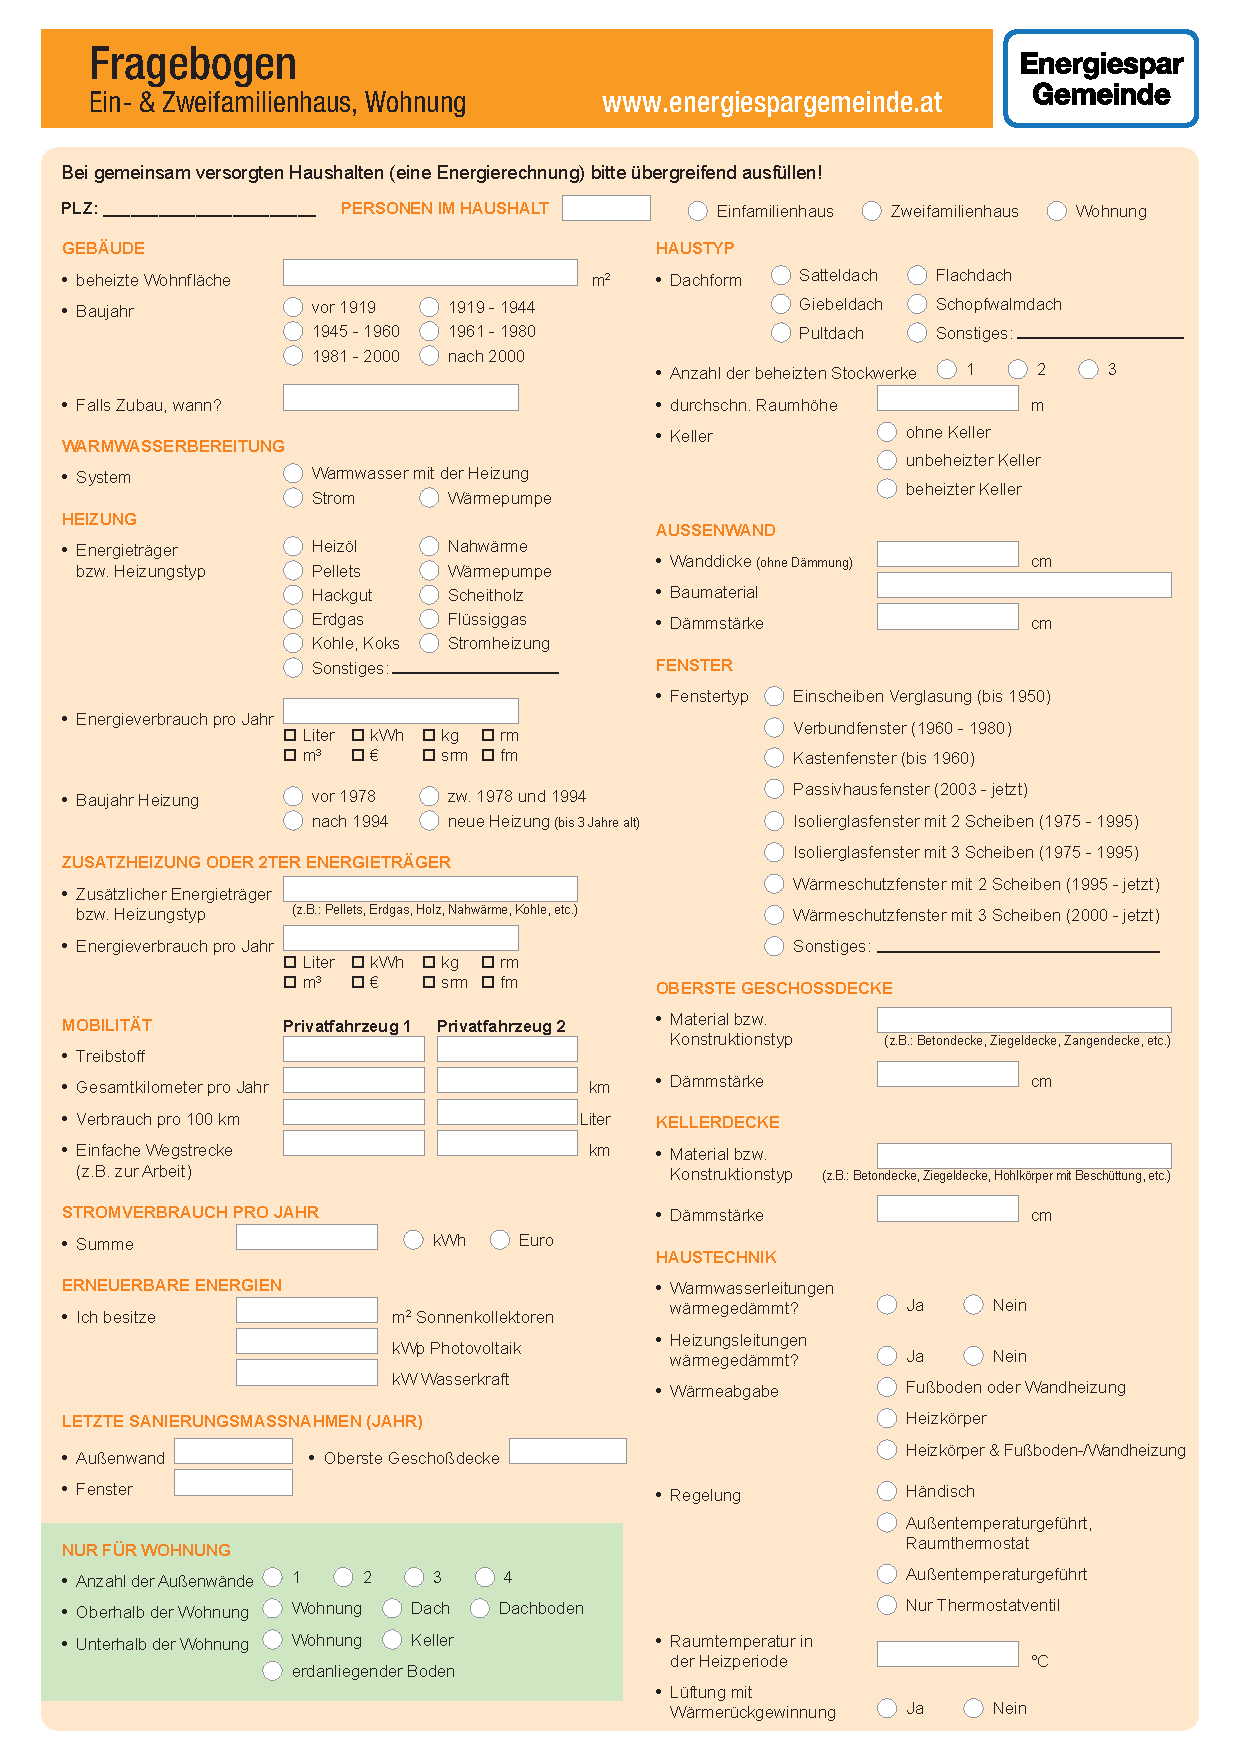
\includepdf[pages=1-,width=\textwidth,frame=true,pagecommand={}]{images/fragebogen}
\end{LaTeXCode}
%
The included pages are automatically scaled to the text width of the \latex document
by \verb!width=\textwidth! and \verb!frame=true! adds a surrounding border.

This example assumes that the external PDF document is in A4 page format.
With other formats you may have to adjust the scaling "manually" if the pages become
too tall (\eg\ with \verb!width=0.9\textwidth!).

It is also important that all \emph{fonts} used in the external PDF document are
correct and fully \emph{embedded}, otherwise the PDF document generated by \latex may
not be viewable in another system environment!


\section{References to Included PDF Pages}

If you want to refer to specific pages in the included PDF, the easiest way is to import
single pages one by one and add a \emph{label} to each, as in this example:
%
\begin{LaTeXCode}[numbers=none]
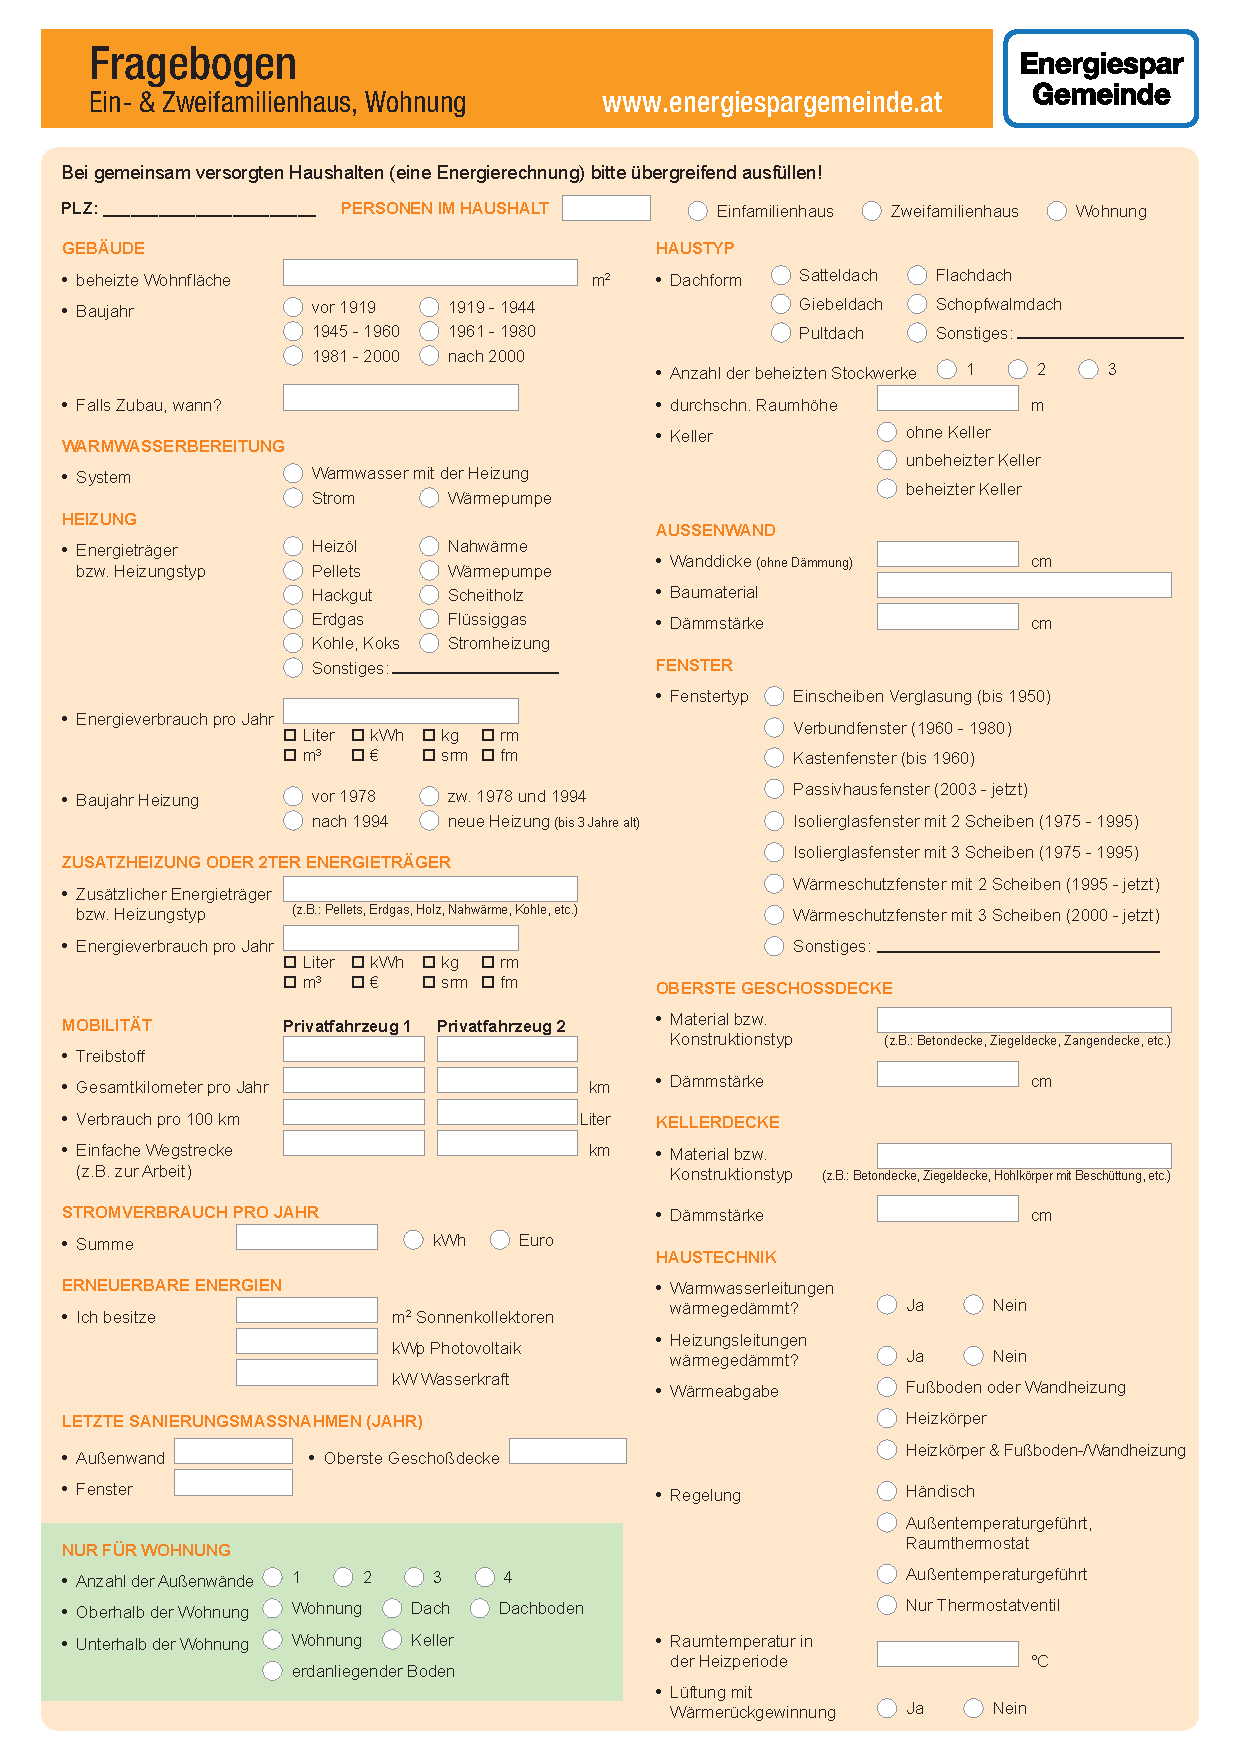
\includepdf[pages=1,width=\textwidth,frame=true,
		pagecommand={\label{PDF1}}]{images/fragebogen}
\includepdf[pages=2,width=\textwidth,frame=true,
		pagecommand={\label{PDF2}}]{images/fragebogen}
\end{LaTeXCode}
%
For example, in this case you could use \verb!\pageref{PDF2}! to specify the current page
number of the 2nd \ page of the included PDF document. 
Many other options (\eg, specifying page intervals) can be found in the detailed documentation
for the \texttt{pdfpages} package.

% And here the foreign PDF document actually included:
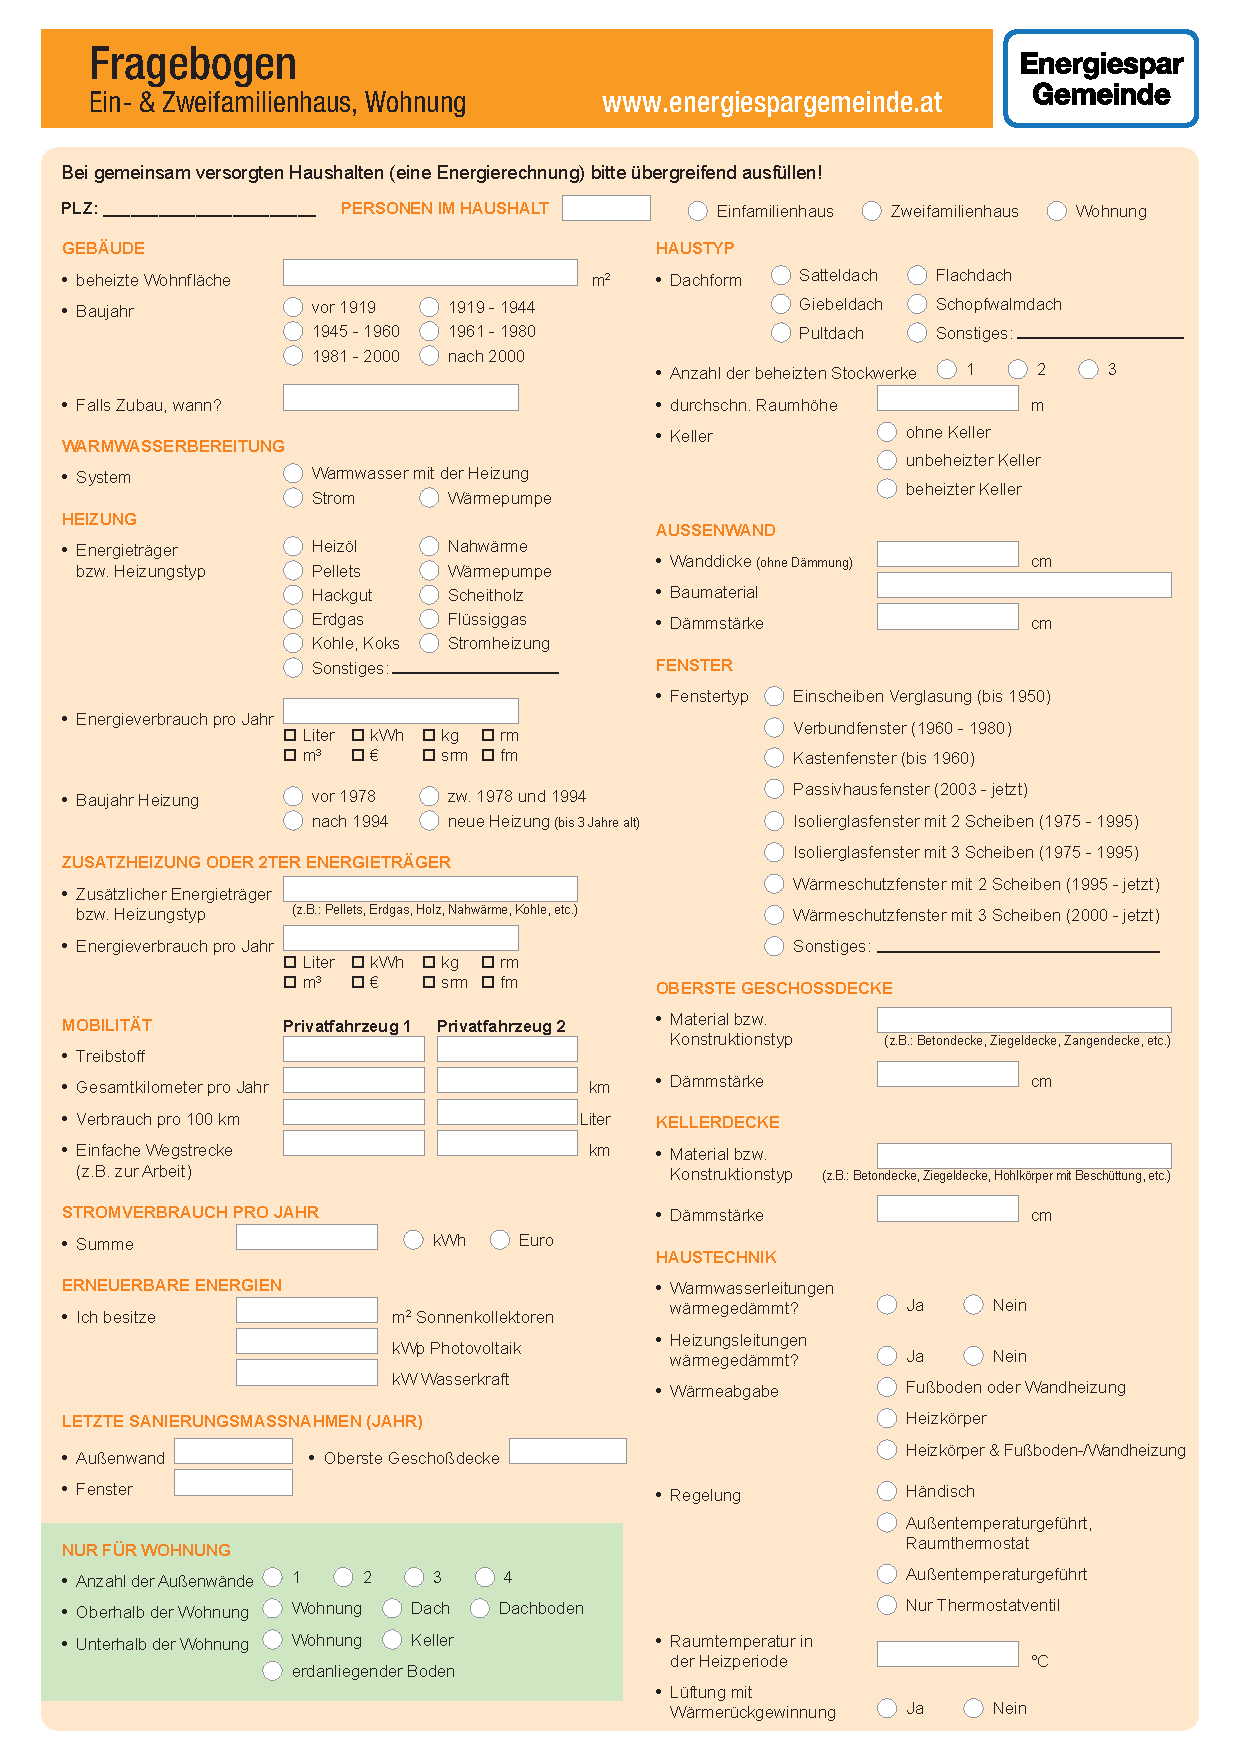
\includepdf[pages=1-,width=\textwidth,frame=true,pagecommand={}]{images/fragebogen}



 % Included other PDF document
\chapter{\latex-Quellcode}
\label{app:latex}

\section*{Hauptdatei \texttt{main.tex}}

\paragraph{Anmerkung:}
Das sollte nur ein \emph{Beispiel} für die Einbindung von Quellcode
in einem Anhang sein. Die dazu verwendeten Anweisungen sind folgende:
%
\begin{LaTeXCode}[numbers=none]
\begin{footnotesize}
\verbatiminput{main.tex}
\end{footnotesize}
\end{LaTeXCode}
%
Natürlich ist der \latex-Quellcode der eigenen Abschlussarbeit meist
\emph{nicht} interessant genug, um ihn hier wiederzugeben!

\begin{footnotesize}
\verbatiminput{main.tex}
\end{footnotesize}





 % Source text of this document

%%%-----------------------------------------------------------------------------
\backmatter                           % Back part (bibliography, glossary, etc.)
%%%-----------------------------------------------------------------------------

\MakeBibliography % References

%%%-----------------------------------------------------------------------------
% Special page for checking print size
%%%-----------------------------------------------------------------------------

\chapter*{Check Final Print Size}

\begin{center}
{\Large --- Check final print size! ---}

\bigskip

\calibrationbox{100}{50} % width/height of box in mm

\bigskip

{\Large --- Remove this page after printing! ---}

\end{center}



%%%-----------------------------------------------------------------------------
\end{document}
%%%-----------------------------------------------------------------------------
